\documentclass{beamer}
\usetheme{madrid}

\usepackage{ctex}
\usepackage{color}
\usepackage{tikz}
\usetikzlibrary{positioning, shapes.geometric}
\usepackage{graphicx}

\usepackage{advdate}
\usepackage{subfigure}
\usepackage{booktabs}

\usepackage{cite}
\usepackage{amsmath}

\hypersetup{pdfpagemode=FullScreen}

\title{空间辐射场三维重构方法}
\author[刘铭]{%
    刘铭 \\
    指导老师:宋玉收%
}
\institute{哈尔滨工程大学核科学与技术学院}
\date{%\AdvanceDate[+1]
\today}

\begin{document}

\begin{frame}
    \maketitle
\end{frame}

\begin{frame}
    \tableofcontents
\end{frame}

\section{论文摘要}

\subsection{论文研究意义}
\begin{frame}
    \frametitle{论文研究意义}

    \begin{figure}
        \centering
        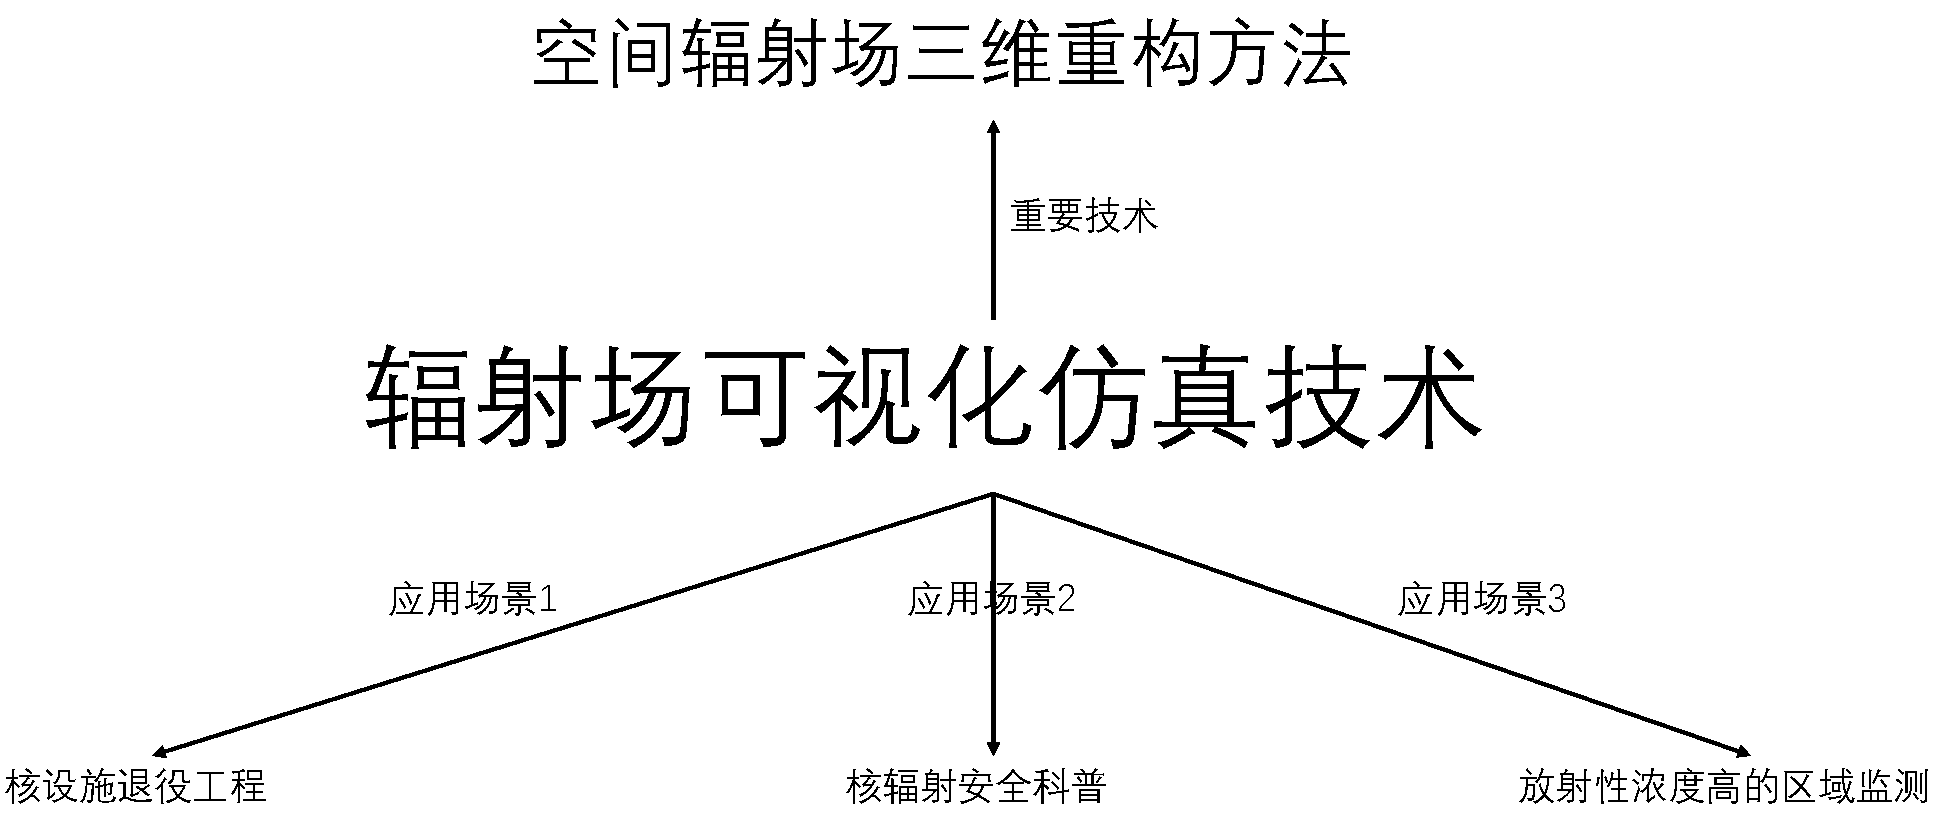
\includegraphics[width=1.0\textwidth]{figures/研究意义.pdf}
    \end{figure}

\end{frame}

\subsection{论文研究工作}
\begin{frame}
    \frametitle{论文研究工作}
    \begin{enumerate}
        \item 提出一种基于多层B样条插值算法和克里金插值算法的辐射场插值重构方法
        \item 利用Geant4设计并构建四种类型的辐射场模型,验证该方法的可行性
        \item 将本论文提出的插值重构算法与多层B样条插值、克里金插值方法进行比较
    \end{enumerate}
\end{frame}

\section{研究背景}

\subsection{重构方法}
\begin{frame}
    \frametitle{重构方法}
    辐射场重构方法主要分为正演法和反演法
\end{frame}

\subsection{插值算法}
\begin{frame}
    \frametitle{插值算法}
    按插值区域分类:
    \begin{enumerate}
        \item 整体插值
        \item 局部插值
        \item 边界内插值
    \end{enumerate}
    按插值的标准分类:
    \begin{enumerate}
        \item 确定性插值
        \item 地统计插值
    \end{enumerate}
\end{frame}

\section{理论基础}

\subsection{多层B样条插值}
\begin{frame}
    \frametitle{B样条插值原理}
    B样条方法(Basic Spline)是由Gordon与Riesenfeld在研究贝齐尔方法的基础上引入的,它在计算上具有递推性、规范性、局部支承性(非负性)、可微性等优点。
    \begin{equation}
        f(x,y,z)=\sum_{i=0}^{3}\sum_{j=0}^{3}\sum_{k=0}^{3}B_{i}(r)B_{j}(s)B_{k}(t) \phi_{(a+i)(b+j)(c+k)}
        \label{三次B样条插值函数}
    \end{equation}
    其中,$ B(t) $为基函数,其计算公式为:
    \begin{equation*}
        B_{0} \left( t \right) = \left( 1 - t \right)^{3} / 6
    \end{equation*}
    \begin{equation*}
        B_{1} \left( t \right) = \left( 3 t^{3} - 6 t^{2} + 4 \right) / 6
    \end{equation*}
    \begin{equation*}
        B_{2} \left( t \right) = \left( -3 t^{3} + 3 t^{2}  + 3 t + 1 \right) / 6
    \end{equation*}
    \begin{equation*}
        B_{3} \left( t \right) = t^{3} / 6
    \end{equation*}
\end{frame}

\begin{frame}
    \frametitle{B样条插值原理}
    为了确定控制栅格$ \Phi $,首先考虑离散数据点集$ \mathbf{P} $中的一个数据点$ \left( x_{c}, y_{c}, z_{c}, v_{c} \right) $,由三次样条插值公式\ref{三次B样条插值函数}可知,样条函数值$ f\left( x_{c}, y_{c}, z_{c} \right) $与其相邻的64个控制点$ \left( x_{c}, y_{c}, z_{c} \right) $相关。
    \begin{equation}
        v_{c} = \sum_{i=0}^{3}\sum_{j=0}^{3}\sum_{k=0}^{3} w_{ijk} \phi_{ijk}
        \label{控制点约束公式}
    \end{equation}
    存在许多组控制点数据$ \phi_{ijk} $满足公式\ref{控制点约束公式},为了使插值函数$ f $在定义域上偏差最小化,选取一组最小二乘最小的数$ \sum_{i=0}^{3}\sum_{j=0}^{3}\sum_{k=0}^{3} \phi_{ijk}^{2} $作为控制点(这将对多层B样条插值有利)。可推导出控制点方程为:
    \begin{equation}
        \phi_{ijk} = \frac{w_{ijk}v_{c}}{\sum_{d=0}^{3}\sum_{e=0}^{3}\sum_{g=0}^{3}w_{deg}^{2}}
        \label{控制点方程}
    \end{equation}
\end{frame}

\begin{frame}
    \frametitle{B样条插值原理}
    设$ P_{ijk} $为控制点$ \phi_{ijk} $的临近数据集,则:
    \begin{equation*}
        P_{ijk} = \{ \left( x_{c}, y_{c}, z_{c}, v_{c} \right) \in \mathbf{P} | i-2 \leq x_{c} < i+2, j-2 \leq y_{c} < j+2, k-2 \leq z_{c} < k+2 \}
    \end{equation*}

    对于每个散乱数据点$ P_{ijk} = \left( x_{c}, y_{c}, z_{c},v_{c} \right) $,由公式\ref{控制点方程}可以得出控制点$ \phi_{ijk} $的值$ \phi_{c} $:
    \begin{equation}
        \phi_{c} = \frac{w_{c}v_{c}}{\sum_{d=0}^{3}\sum_{e=0}^{3}\sum_{g=0}^{3}w_{deg}^{2}}
    \end{equation}
\end{frame}

\begin{frame}
    \frametitle{B样条插值原理}
    最终计算选取误差$ e\left( \phi_{ijk} \right) = \sum_{c}\left( w_{c}\phi_{ijk} - w_{c}\phi_{c} \right)^{2} $最小的值作为控制点值$ \phi_{ijk} $,其中$ \left( w_{c}\phi_{ijk} - w_{c}\phi_{c} \right) $是控制点$ \phi_{ijk} $对插值函数$ f $在$ \left( x_{c}, y_{c}, z_{c} \right) $实际权重与真实权重之差。

    $ e_{\phi_{ijk}} $是控制点$ \phi_{ijk} $的近似误差,用不同数据点对该控制点的权重来计算控制点值,可以得到:
    \begin{equation}
        \phi_{ijk} = \frac{\sum_{c}w_{c}^{2}\phi_{c}}{\sum_{c}w_{c}^{2}}
        \label{临近控制点计算方程}
    \end{equation}
\end{frame}

\begin{frame}
    \frametitle{B样条插值算法}
    \begin{figure}[htbp]
        \centering
        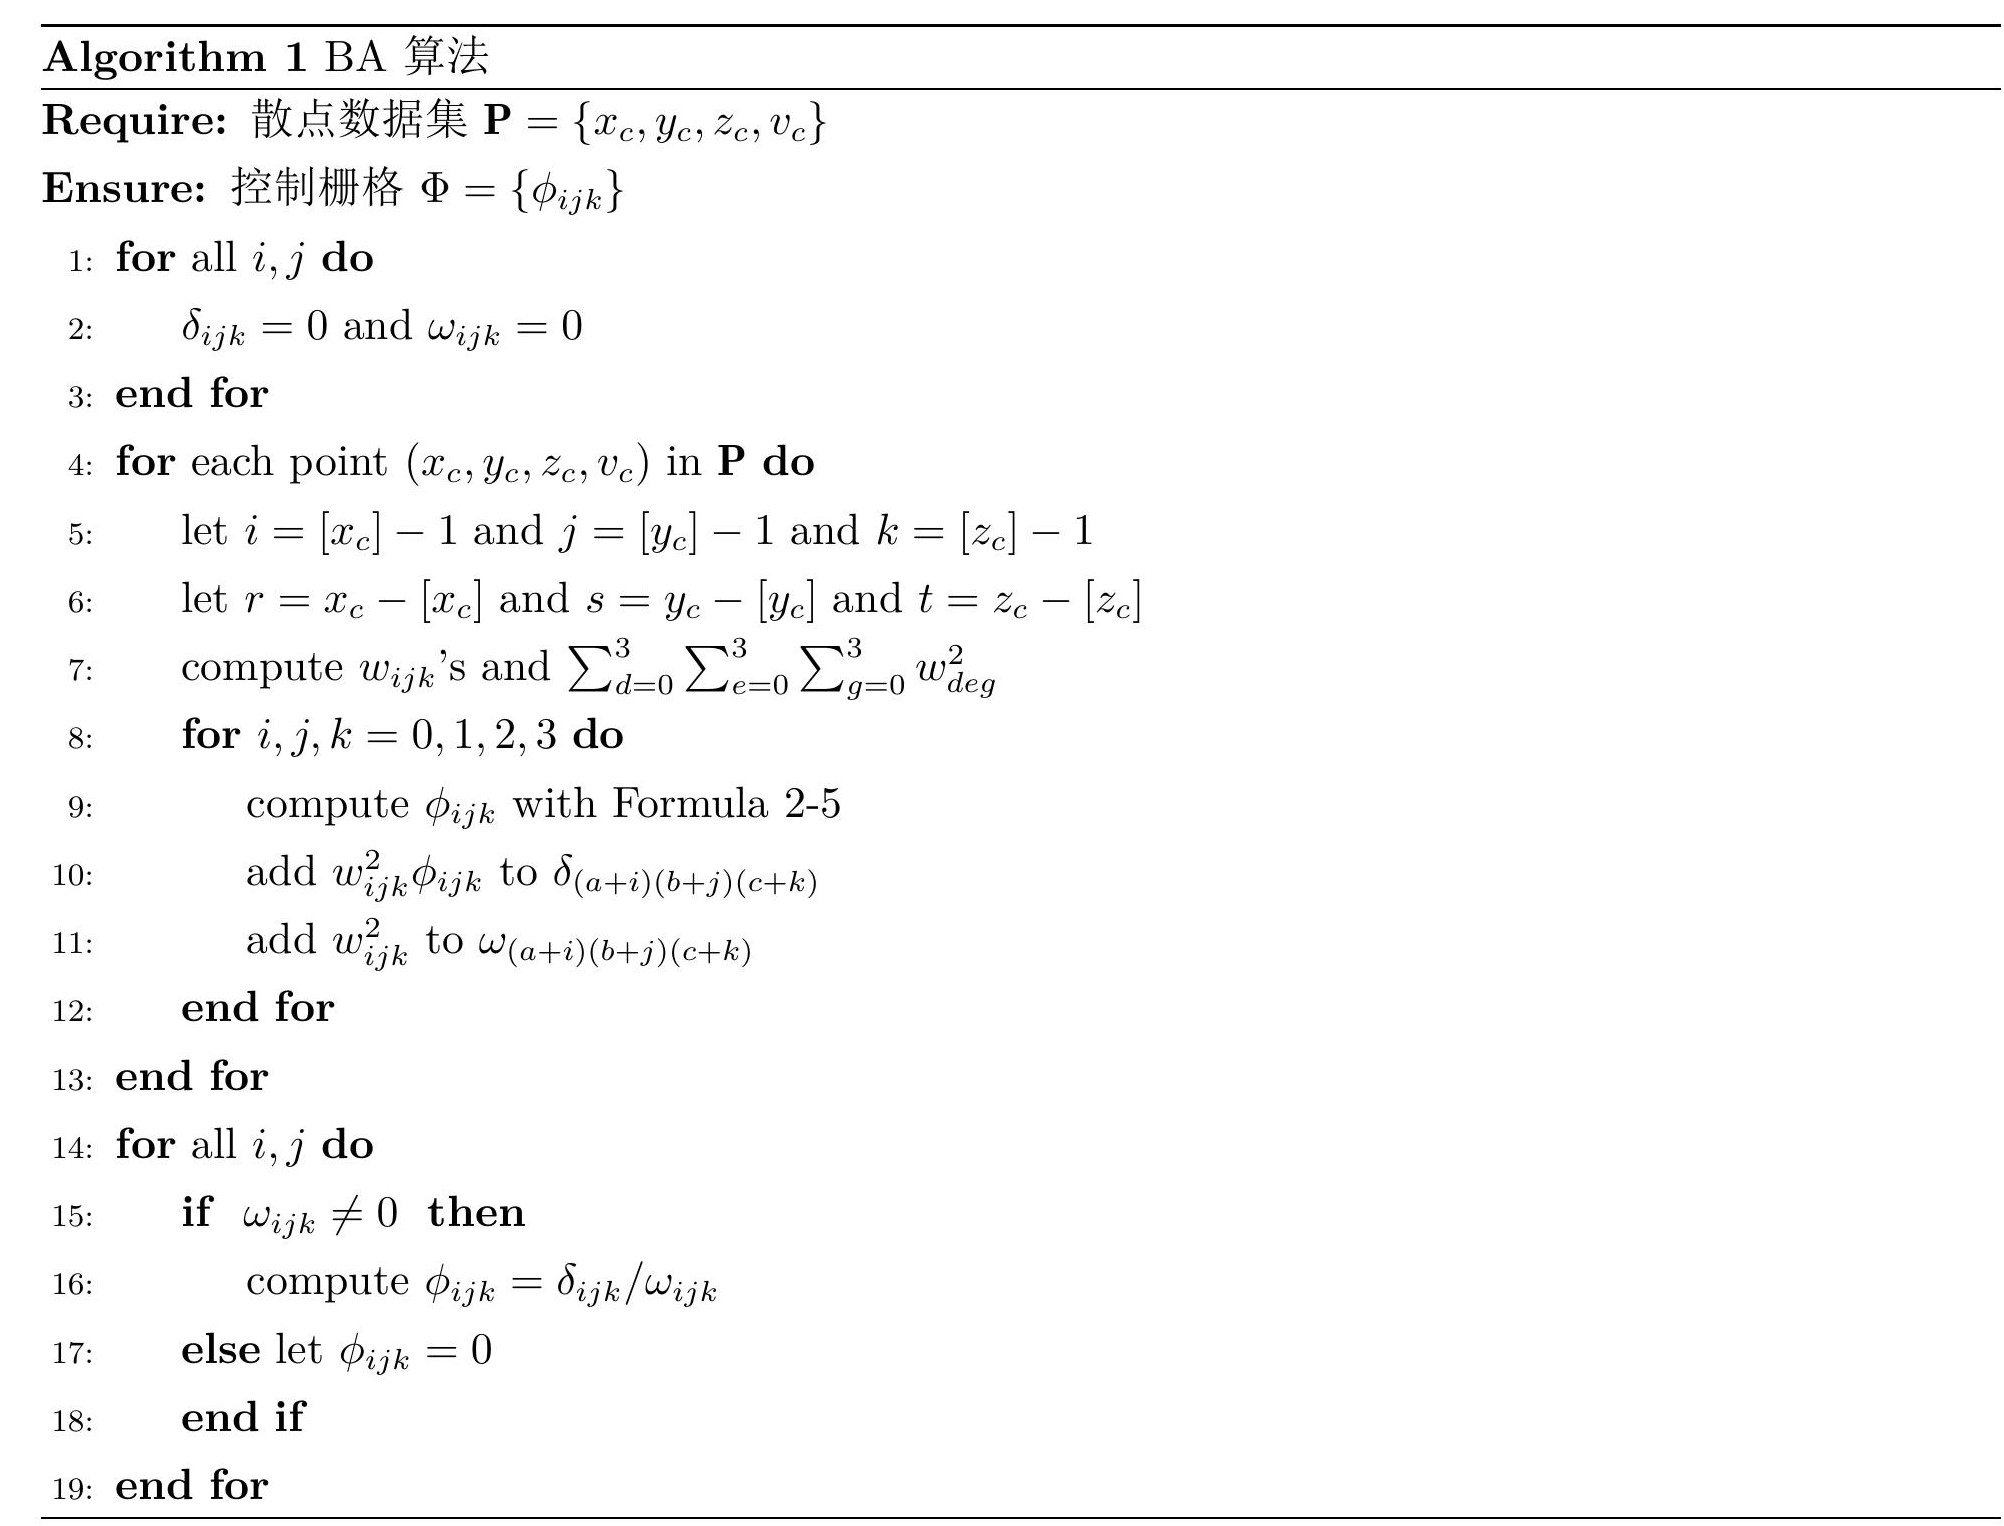
\includegraphics[height=0.85\textheight]{figures/BA算法.jpg}
    \end{figure}
\end{frame}

\begin{frame}
    \frametitle{多层B样条插值原理}
    通过BA算法生成的插值函数在形状平滑度和精度之间存在折衷,因此,提出多层B样条插值算法来避免这种折衷。多层B样条算法通过控制栅格的多层结构来生成插值函数$ f_{k} $序列,对插值函数序列$ f_{k} $每个函数进行加和,得到最终插值函数。在该序列中,来自稀疏栅格的函数提供初略的近似,该近似在精度上被来自更精细栅格的函数进一步细化,最终将这些函数的和减少到一个等价的B样条函数。
    \begin{eqnarray}
        f = \sum_{k=0}^{h} f_{k}
    \end{eqnarray}

    对于第$ k $层,使用近似差数据集$ \mathbf{P_{k}} = \{ \left( x_{c}, y_{c}, z_{c}, \bigtriangleup^{k}v_{c} \right) \} $计算出第$ k $层控制栅格$ \Phi_{k} $,从而推导近似函数$ f_{k} $,其中$ \bigtriangleup^{k}v_{c} = v_{c} - \sum_{i=0}^{k-1}f_{i}\left( x_{c}, y_{c}, z_{c} \right) = \bigtriangleup^{k-1}v_{c} - f_{k-1}\left( x_{c}, y_{c}, z_{c} \right) , \bigtriangleup^{0}v_{c} = v_{c} $
\end{frame}

\begin{frame}
    \frametitle{多层B样条插值算法}
    \begin{figure}
        \centering
        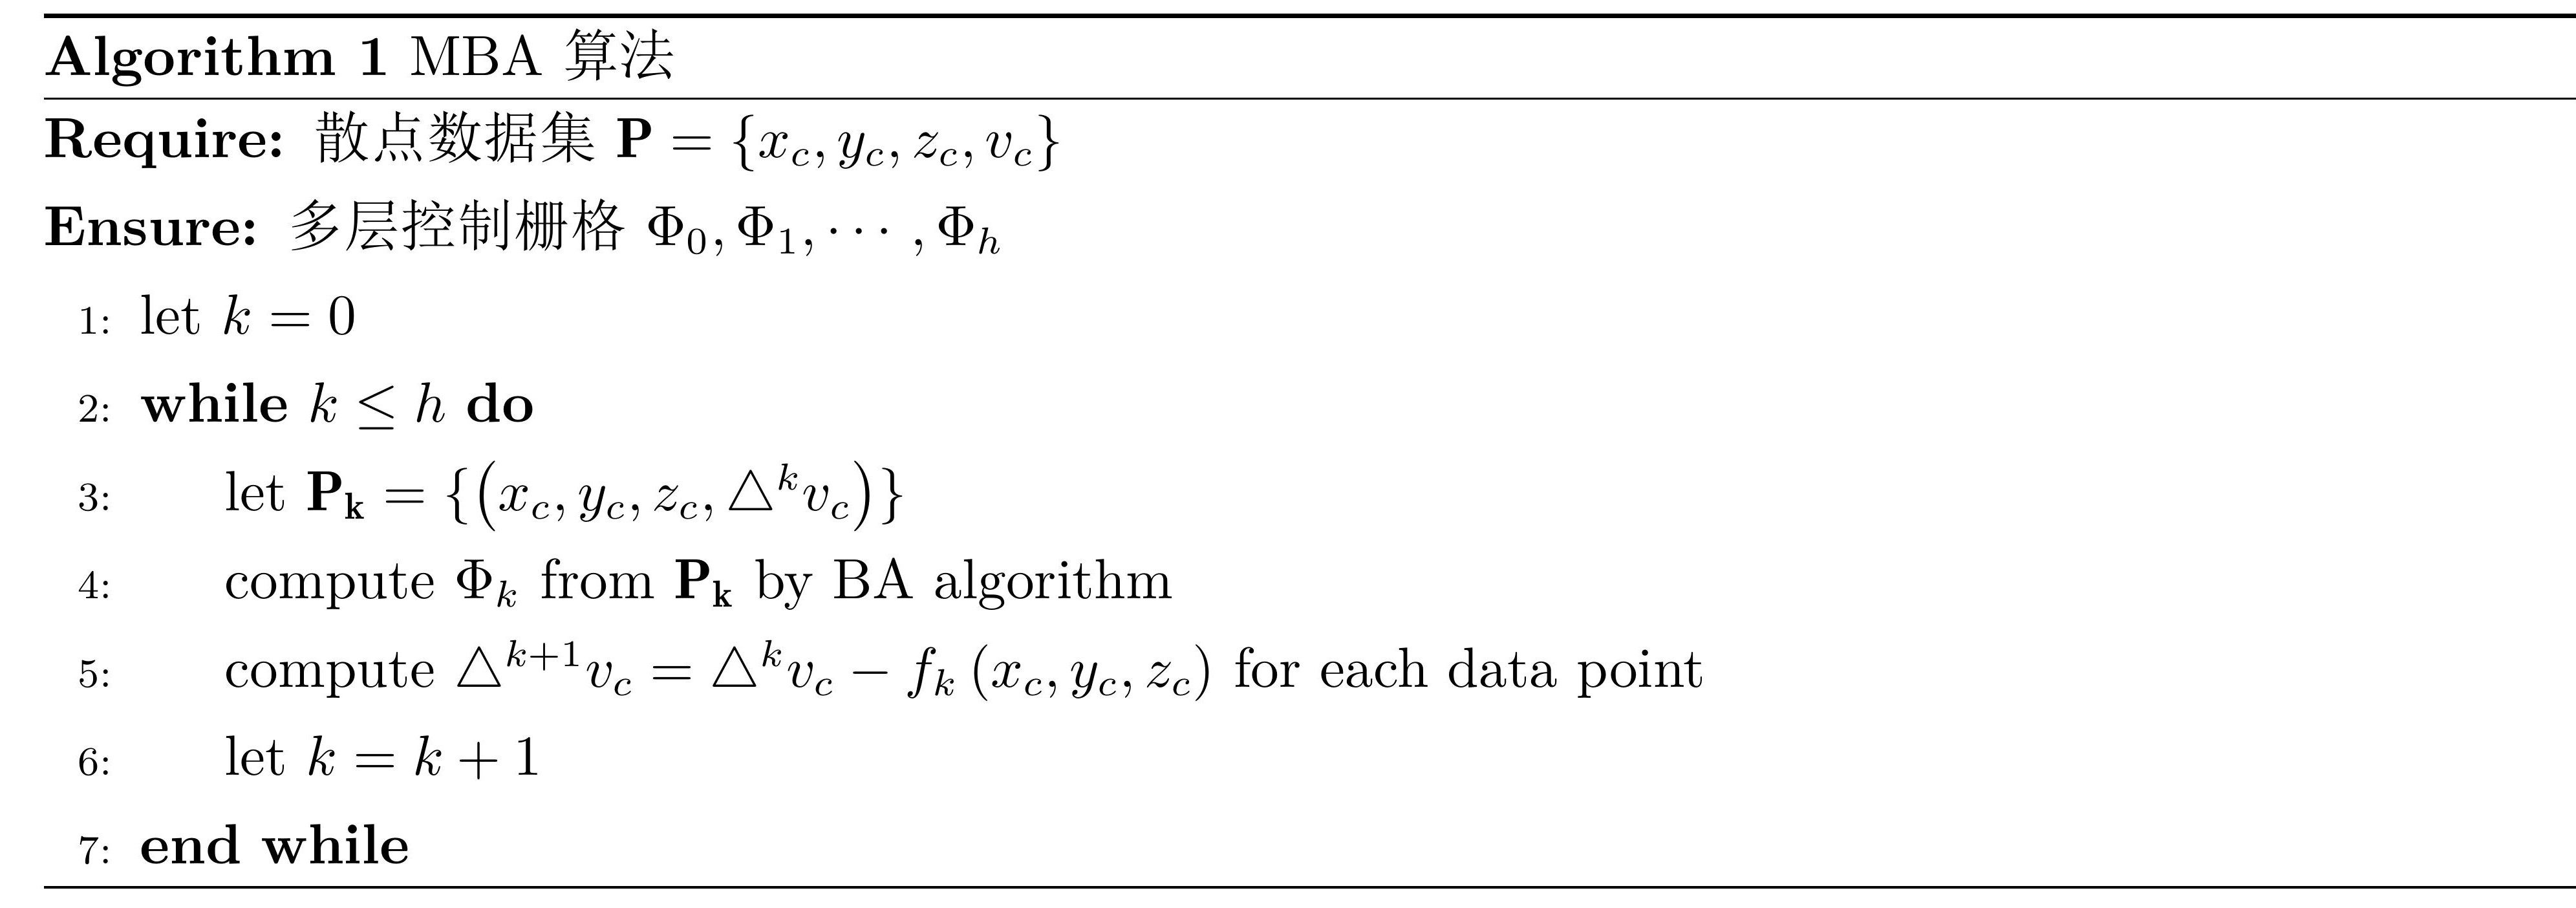
\includegraphics[height=0.70\textheight]{figures/MBA算法.jpg}
    \end{figure}
\end{frame}

\begin{frame}
    \frametitle{多层B样条插值优化原理}
    MBA算法的时间复杂度为$ O\left( p+mnl \right) + O\left( p+\frac{1}{8}mnl \right)+ \cdots+O\left( p+\frac{1}{8^{h}}mnl \right) = O\left( hp+\frac{8}{7}mnl \right) $ \\
    空间复杂度为$ O\left( p+\frac{8}{7}mnl \right) $

    \vspace*{1cm}
    通过在控制栅格中逐步应用B样条优化来解决复杂度高的问题,使得$ f $可以用一个B样条函数来表示,而不是几个B样条函数之和。因此,$ f_{k} $的计算仅在$ \Phi_{k} $中少量的控制点,而不是$ \Omega $中的所有点。
\end{frame}

\begin{frame}
    \frametitle{多层B样条插值优化算法}
    \begin{figure}
        \centering
        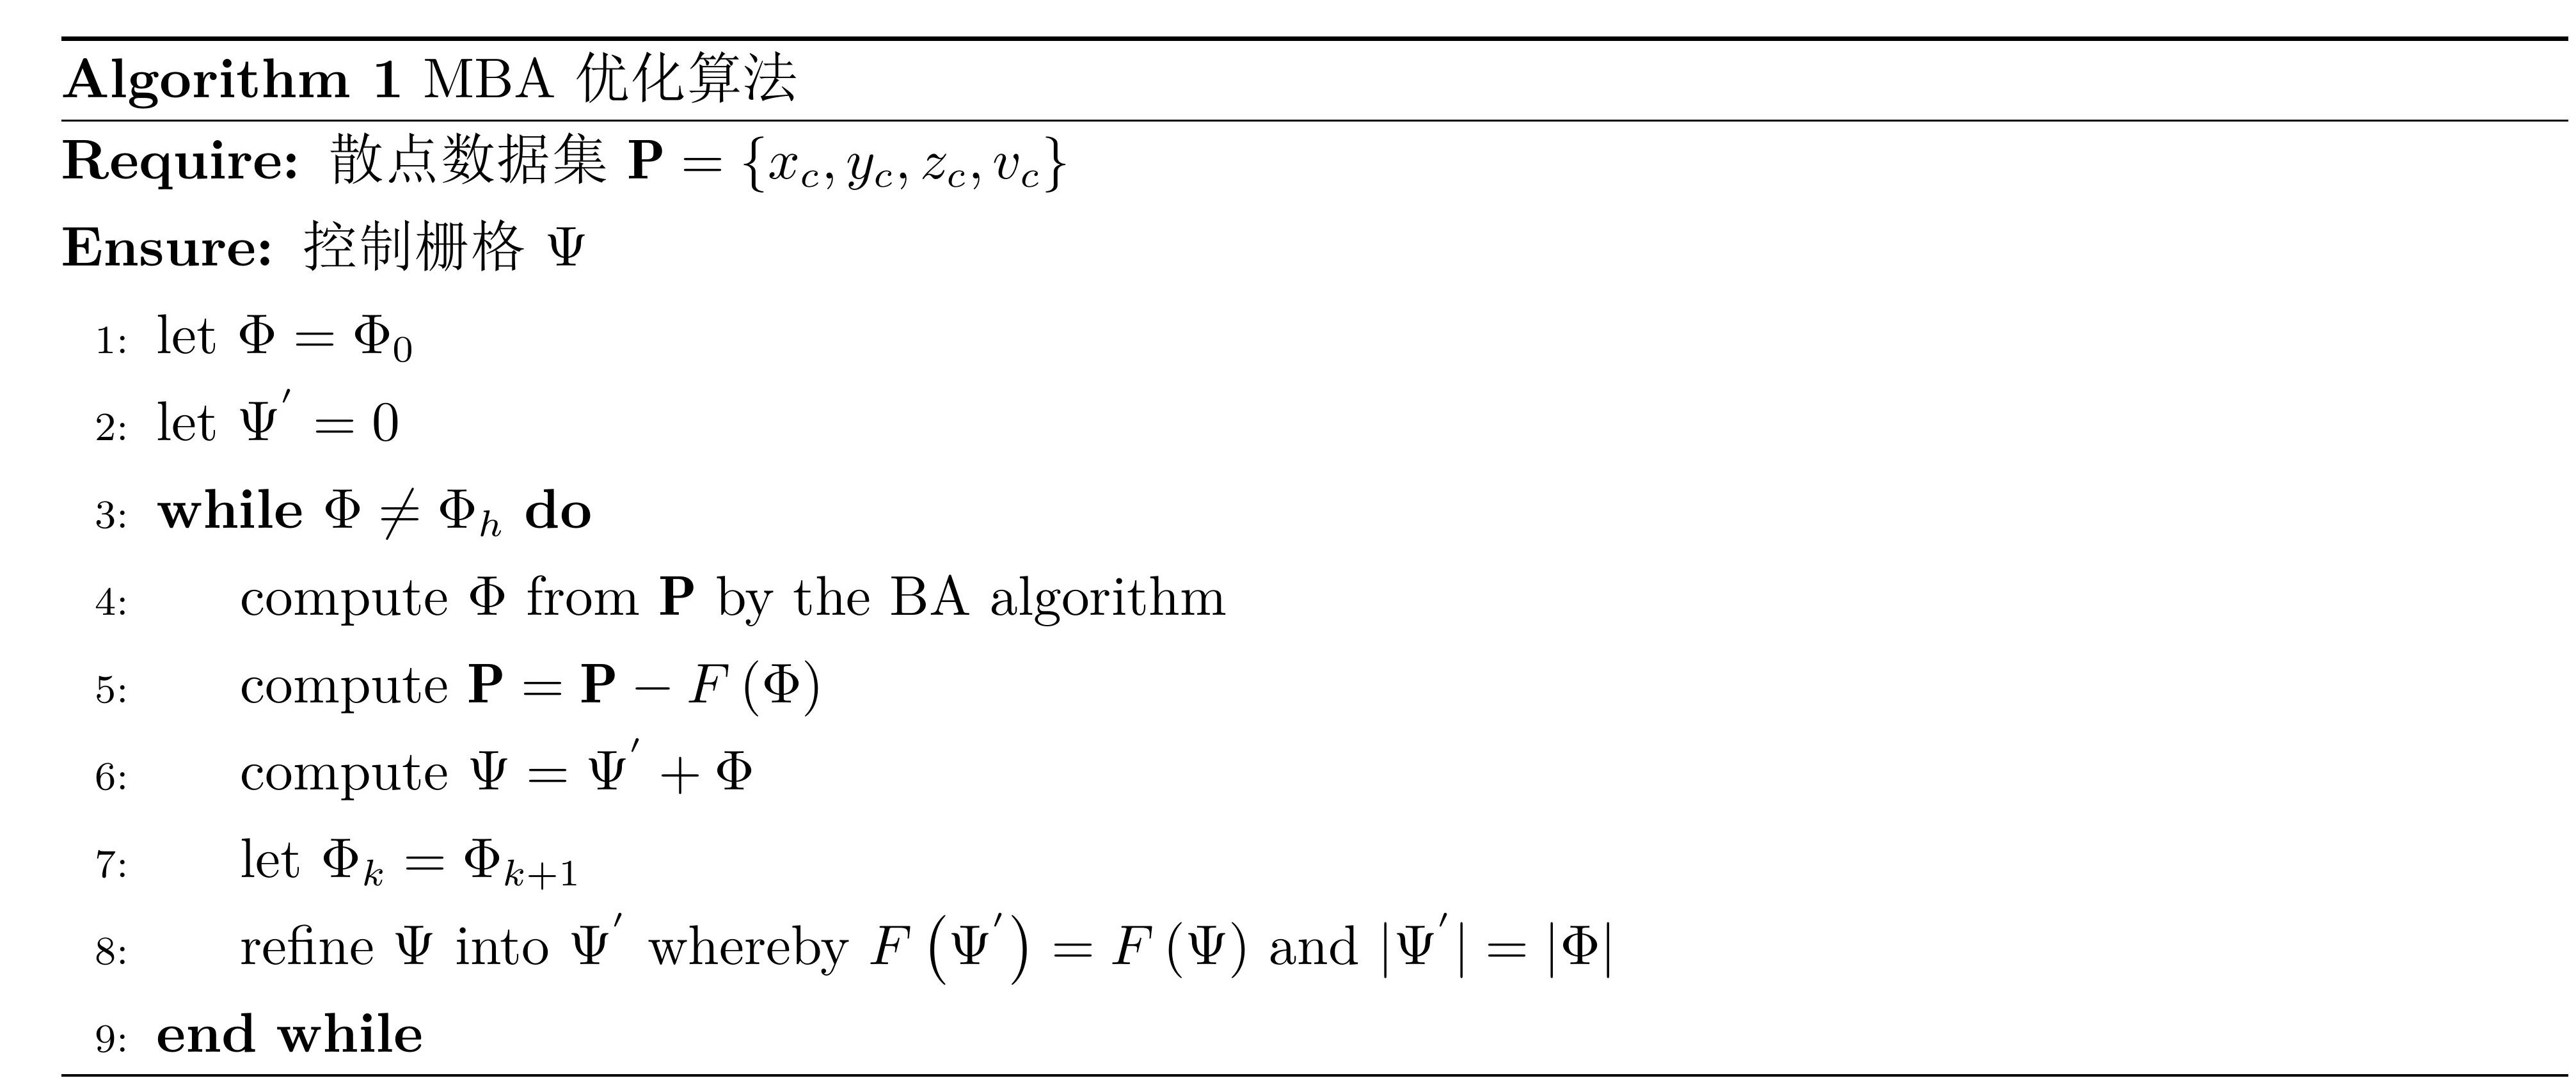
\includegraphics[height=0.7\textheight]{figures/MBA优化算法.jpg}
    \end{figure}

    时间复杂度为$ O\left( hp+\frac{8}{7}mnl \right) $,空间复杂度为$ O\left( p+mnl \right) $
\end{frame}

\subsection{克里金插值}
\begin{frame}
    \frametitle{克里金插值原理}
    假设有$ N $个随机变量$ V $的值已经记录在采样点$ \mathbf{s}_{1}, \mathbf{s}_{2}, \mathbf{s}_{3} , \cdots , \mathbf{s}_{N} $作为已知点,对于克里金插值,我们通过以下公式预测其插值点$ \mathbf{s}_{0} $的值:
    \begin{equation}
        \hat{V}\left( \mathbf{s}_{0} \right) = \sum_{i=1}^{N} \lambda_{i} V\left( \mathbf{s}_{i} \right)
        \label{点克里金插值公式}
    \end{equation}

    为了确保估计值无偏以及权重之和为1,有:
    \begin{equation}
        E\left[ \hat{V}\left( \mathbf{s}_{0} \right) - V\left( \mathbf{s}_{0} \right) \right] = 0
        \label{点克里金插值无偏}
    \end{equation}
    \begin{equation}
        \sum_{i=1}^{N} \lambda_{i} = 1
        \label{点克里金插值权重之和为1}
    \end{equation}
\end{frame}

\begin{frame}
    \frametitle{克里金插值原理}
    预测方差为:
    \begin{equation}
        \begin{split}
            Var\left[ \hat{V} \left( \mathbf{s}_{0} \right) \right]
            & = E\left[ {\hat{V}\left( \mathbf{s}_{0} \right) - V\left( \mathbf{s}_{0} \right)}^{2} \right]     \\
            & = 2 \sum_{i=1}^{N} \lambda_{i} \gamma\left( \mathbf{s}_{i} - \mathbf{s}_{0} \right) - \sum_{i=1}^{N} \sum_{j=1}^{N} \lambda_{i} \lambda_{j} \gamma\left( \mathbf{s}_{i} - \mathbf{s}_{j} \right)
        \end{split}
        \label{点克里金插值预测方差}
    \end{equation}
    其中,函数$ \gamma\left( \mathbf{s}_{i} - \mathbf{s}_{0} \right) $代表采样点$ \mathbf{s}_{i} $和目标预测点$ \mathbf{s}_{0} $之间的半方差函数(也称半变异函数);$ \gamma\left( \mathbf{s}_{i} - \mathbf{s}_{j} \right) $是采样点$ \mathbf{s}_{i} $和$ \mathbf{s}_{j} $之间的半方差函数。
\end{frame}

\begin{frame}
    \frametitle{克里金插值原理}
    要在权重之和为1的约束下,寻找使得预测值方差最小的权重。通过公式\ref{点克里金插值公式}减去\ref{点克里金插值预测方差},可推导出$ N+1 $个公式,其中包含$ N+1 $个未知数:
    \begin{equation}
        \sum_{i=1}^{N} \lambda_{i} \gamma \left( \mathbf{s}_{i} - \mathbf{s}_{j} \right) + \psi \left( \mathbf{s}_{0} \right) = \gamma \left( \mathbf{s}_{j} - \mathbf{s}_{0} \right) \qquad \text{for all $ j $}
        \label{点克里金法N个方程}
    \end{equation}
    \begin{equation}
        \sum_{i=0}^{N}\lambda_{i} = 1
        \label{点克里金法N+1个方程}
    \end{equation}
    其中,$ \psi \left( \mathbf{s}_{0} \right) $为拉格朗日数乘。
\end{frame}

\begin{frame}
    \frametitle{克里金插值原理}
    展开作为方程组形式为:
    \begin{equation}
        \left\{
        \begin{aligned}
            \gamma \left( \mathbf{s}_{1} - \mathbf{s}_{1} \right) \lambda_{1}+ \gamma \left( \mathbf{s}_{1} - \mathbf{s}_{2} \right) \lambda_{2}+\cdots + \gamma \left( \mathbf{s}_{1} - \mathbf{s}_{n} \right) \lambda_{n}-\psi\left( \mathbf{s}_{0} \right)    & = \gamma \left( \mathbf{s}_{1} - \mathbf{s}_{0} \right) \\
            \gamma \left( \mathbf{s}_{2} - \mathbf{s}_{1} \right) \lambda_{1} + \gamma \left( \mathbf{s}_{2} - \mathbf{s}_{2} \right) \lambda_{2} + \cdots + \gamma \left( \mathbf{s}_{2} - \mathbf{s}_{n} \right) \lambda_{n}-\psi\left( \mathbf{s}_{0} \right) & = \gamma \left( \mathbf{s}_{2} - \mathbf{s}_{0} \right) \\                                                                & \cdots                                                  \\
            \gamma \left( \mathbf{s}_{n} - \mathbf{s}_{1} \right) \lambda_{1}+\gamma \left( \mathbf{s}_{n} - \mathbf{s}_{2} \right) \lambda_{2}+\cdots+\gamma \left( \mathbf{s}_{n} - \mathbf{s}_{n} \right)\lambda_{n}-\psi\left( \mathbf{s}_{0} \right)        & = \gamma \left( \mathbf{s}_{n} - \mathbf{s}_{0} \right) \\
            \lambda_{1}+\lambda_{2}+\cdots+\lambda_{n}                                                                                                                                                                                                           & =1
        \end{aligned}
        \right.
        \label{克里金方程线性方程组}
    \end{equation}
\end{frame}

\begin{frame}
    \frametitle{克里金插值原理}
    矩阵的具体形式为:
    \begin{small}
        \begin{equation}
            \left[\begin{array}{ccccc}
                    \gamma \left( \mathbf{s}_{1} - \mathbf{s}_{1} \right) & \gamma \left( \mathbf{s}_{1} - \mathbf{s}_{2} \right) & \cdots & \gamma \left( \mathbf{s}_{1} - \mathbf{s}_{n} \right) & 1      \\
                    \gamma \left( \mathbf{s}_{2} - \mathbf{s}_{1} \right) & \gamma \left( \mathbf{s}_{2} - \mathbf{s}_{2} \right) & \cdots & \gamma \left( \mathbf{s}_{2} - \mathbf{s}_{n} \right) & 1      \\
                    \cdots                                                & \cdots                                                & \cdots & \cdots                                                & \cdots \\
                    \gamma \left( \mathbf{s}_{n} - \mathbf{s}_{1} \right) & \gamma \left( \mathbf{s}_{n} - \mathbf{s}_{2} \right) & \cdots & \gamma \left( \mathbf{s}_{n} - \mathbf{s}_{n} \right) & 1      \\
                    1                                                     & 1                                                     & \cdots & 1                                                     & 0
                \end{array}\right]\left[\begin{array}{c}
                    \lambda_{1} \\
                    \lambda_{2} \\
                    \cdots      \\
                    \lambda_{n} \\
                    -\psi\left( \mathbf{s}_{0} \right)
                \end{array}\right]=\left[\begin{array}{c}
                    \gamma \left( \mathbf{s}_{1} - \mathbf{s}_{0} \right) \\
                    \gamma \left( \mathbf{s}_{2} - \mathbf{s}_{0} \right) \\
                    \ldots                                                \\
                    \gamma \left( \mathbf{s}_{n} - \mathbf{s}_{0} \right) \\
                    1
                \end{array}\right]
        \end{equation}
    \end{small}
\end{frame}

\section{核心内容}

\subsection{辐射场插值重构算法}
\begin{frame}
    \frametitle{算法流程图}
    \begin{tikzpicture}[node distance=4pt]
        \node[draw, rounded corners]                        (start)   {开始};
        \node[draw, below=of start]                         (step 1)  {导入数据};
        \node[draw, below=of step 1]                        (step 2)  {计算Kriging插值重构辐射场};
        \node[draw, below=of step 2]                        (step 3)  {计算Splines插值重构辐射场};
        \node[draw, below=of step 3]                        (step 4)  {计算两个重构辐射场的偏差};
        \node[draw, diamond, aspect=6, below=of step 4]     (choice)  {偏差值是否大于设定值};
        \node[draw, right=10pt of choice]                   (step x)  {添加测量数据};
        \node[draw, below=10pt of choice]                   (step 5)  {绘制空间辐射场};
        \node[draw, below=of step 5]                        (step 6)  {计算整体偏差};
        \node[draw, rounded corners, below=of step 6]       (end)     {结束};

        \draw[->] (start)  -- (step 1);
        \draw[->] (step 1) -- (step 2);
        \draw[->] (step 2) -- (step 3);
        \draw[->] (step 3) -- (step 4);
        \draw[->] (step 4) -- (choice);
        \draw[->] (choice) -- (step 5);
        \draw[->] (choice) -- node[left]  {否} (step 5);
        \draw[->] (choice) -- node[above] {是}  (step x);
        \draw[->] (step 5) -- (step 6);
        \draw[->] (step x) -- (step x|-step 1) -> (step 1);
        \draw[->] (step 6) -- (end);
    \end{tikzpicture}
\end{frame}

\subsection{辐射场插值重构模块}
\begin{frame}
    \frametitle{模块化设计}
    \begin{figure}
        \centering
        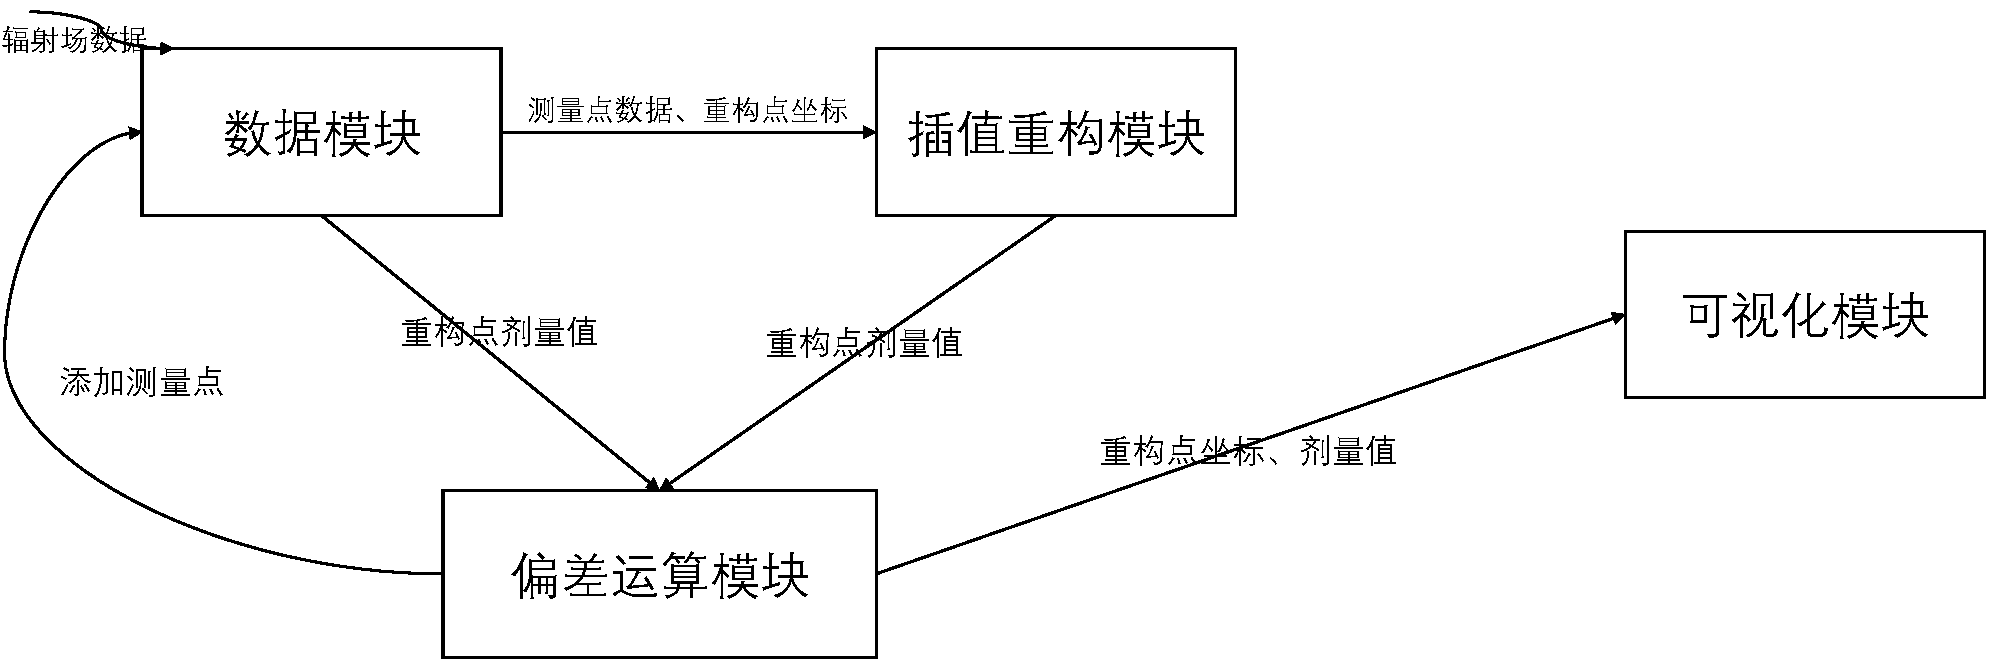
\includegraphics[width=1.0\textwidth]{figures/辐射场重构程序模块.pdf}
    \end{figure}
\end{frame}

\section{成果展示}

\subsection{辐射场重构方法评价}
\begin{frame}
    \frametitle{Geant4模拟辐射场}
    \begin{figure}[htbp]
        \centering
        \subfigure[单点源无屏蔽]{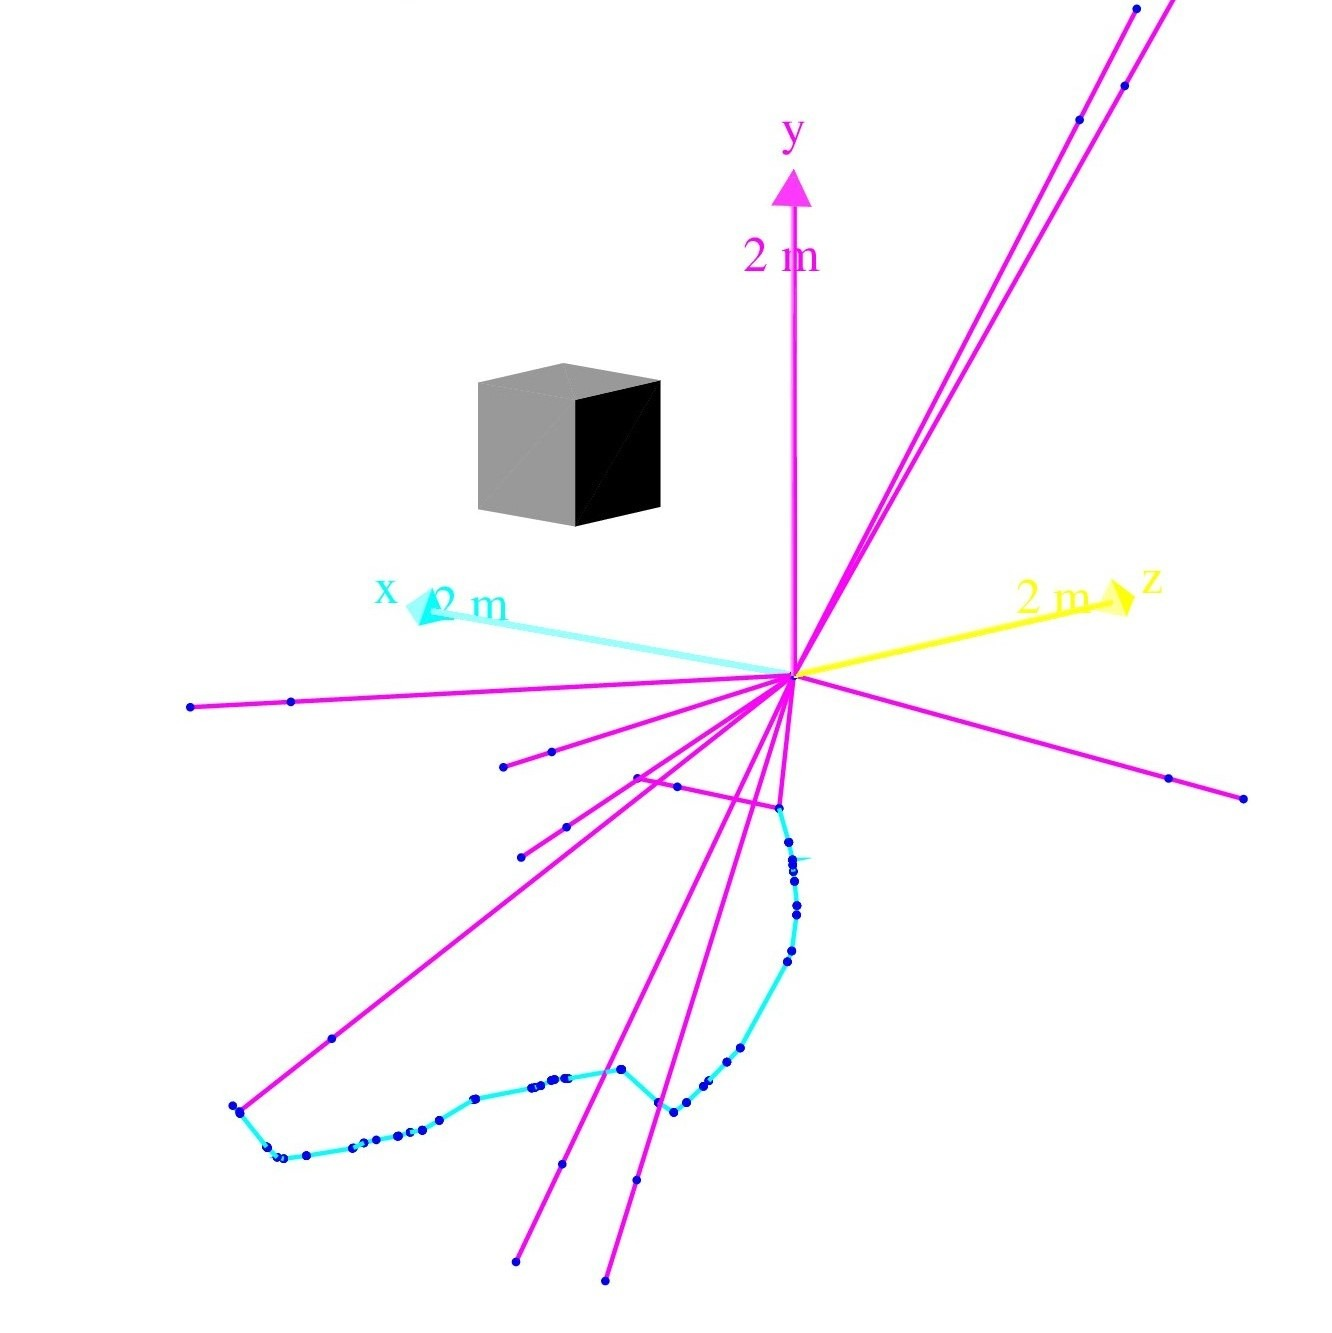
\includegraphics[width=0.24\textwidth]{figures/Geant4/SingleSource.jpg}\label{fig:exph1}}
        \subfigure[单点源有屏蔽]{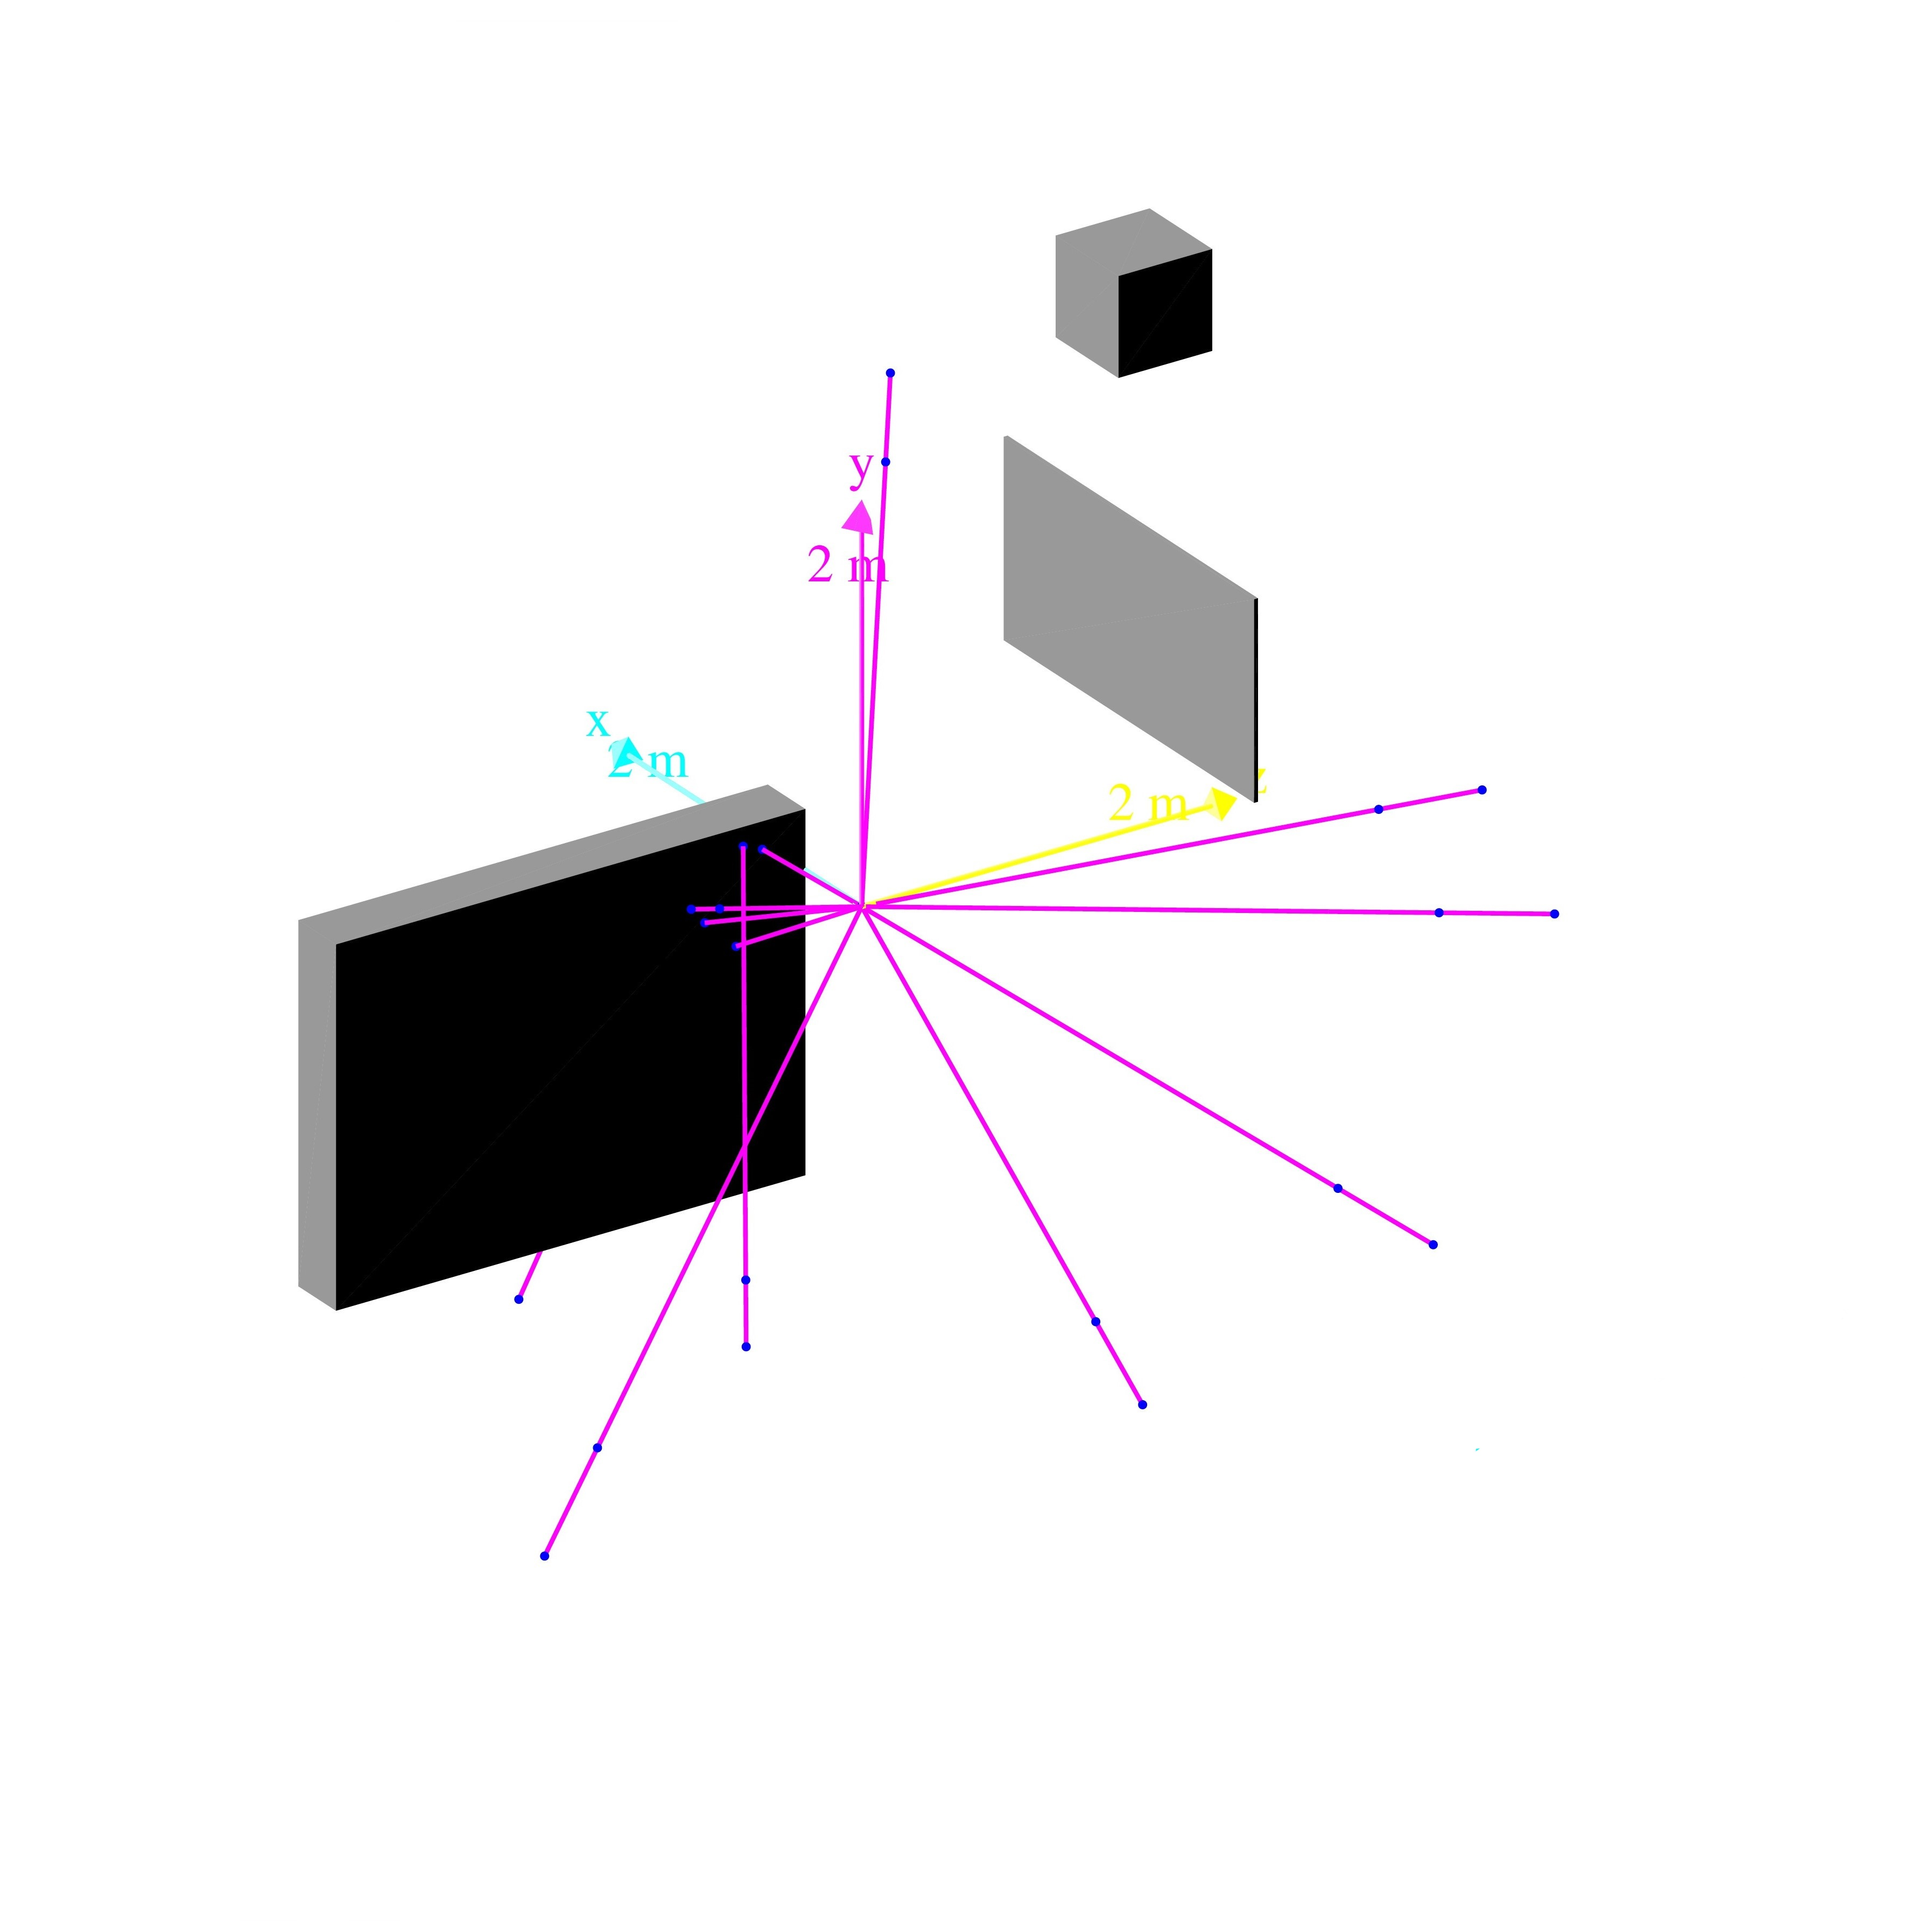
\includegraphics[width=0.24\textwidth]{figures/Geant4/SingleSourceShield.jpg}\label{fig:exgr1}}

        \subfigure[多点源无屏蔽]{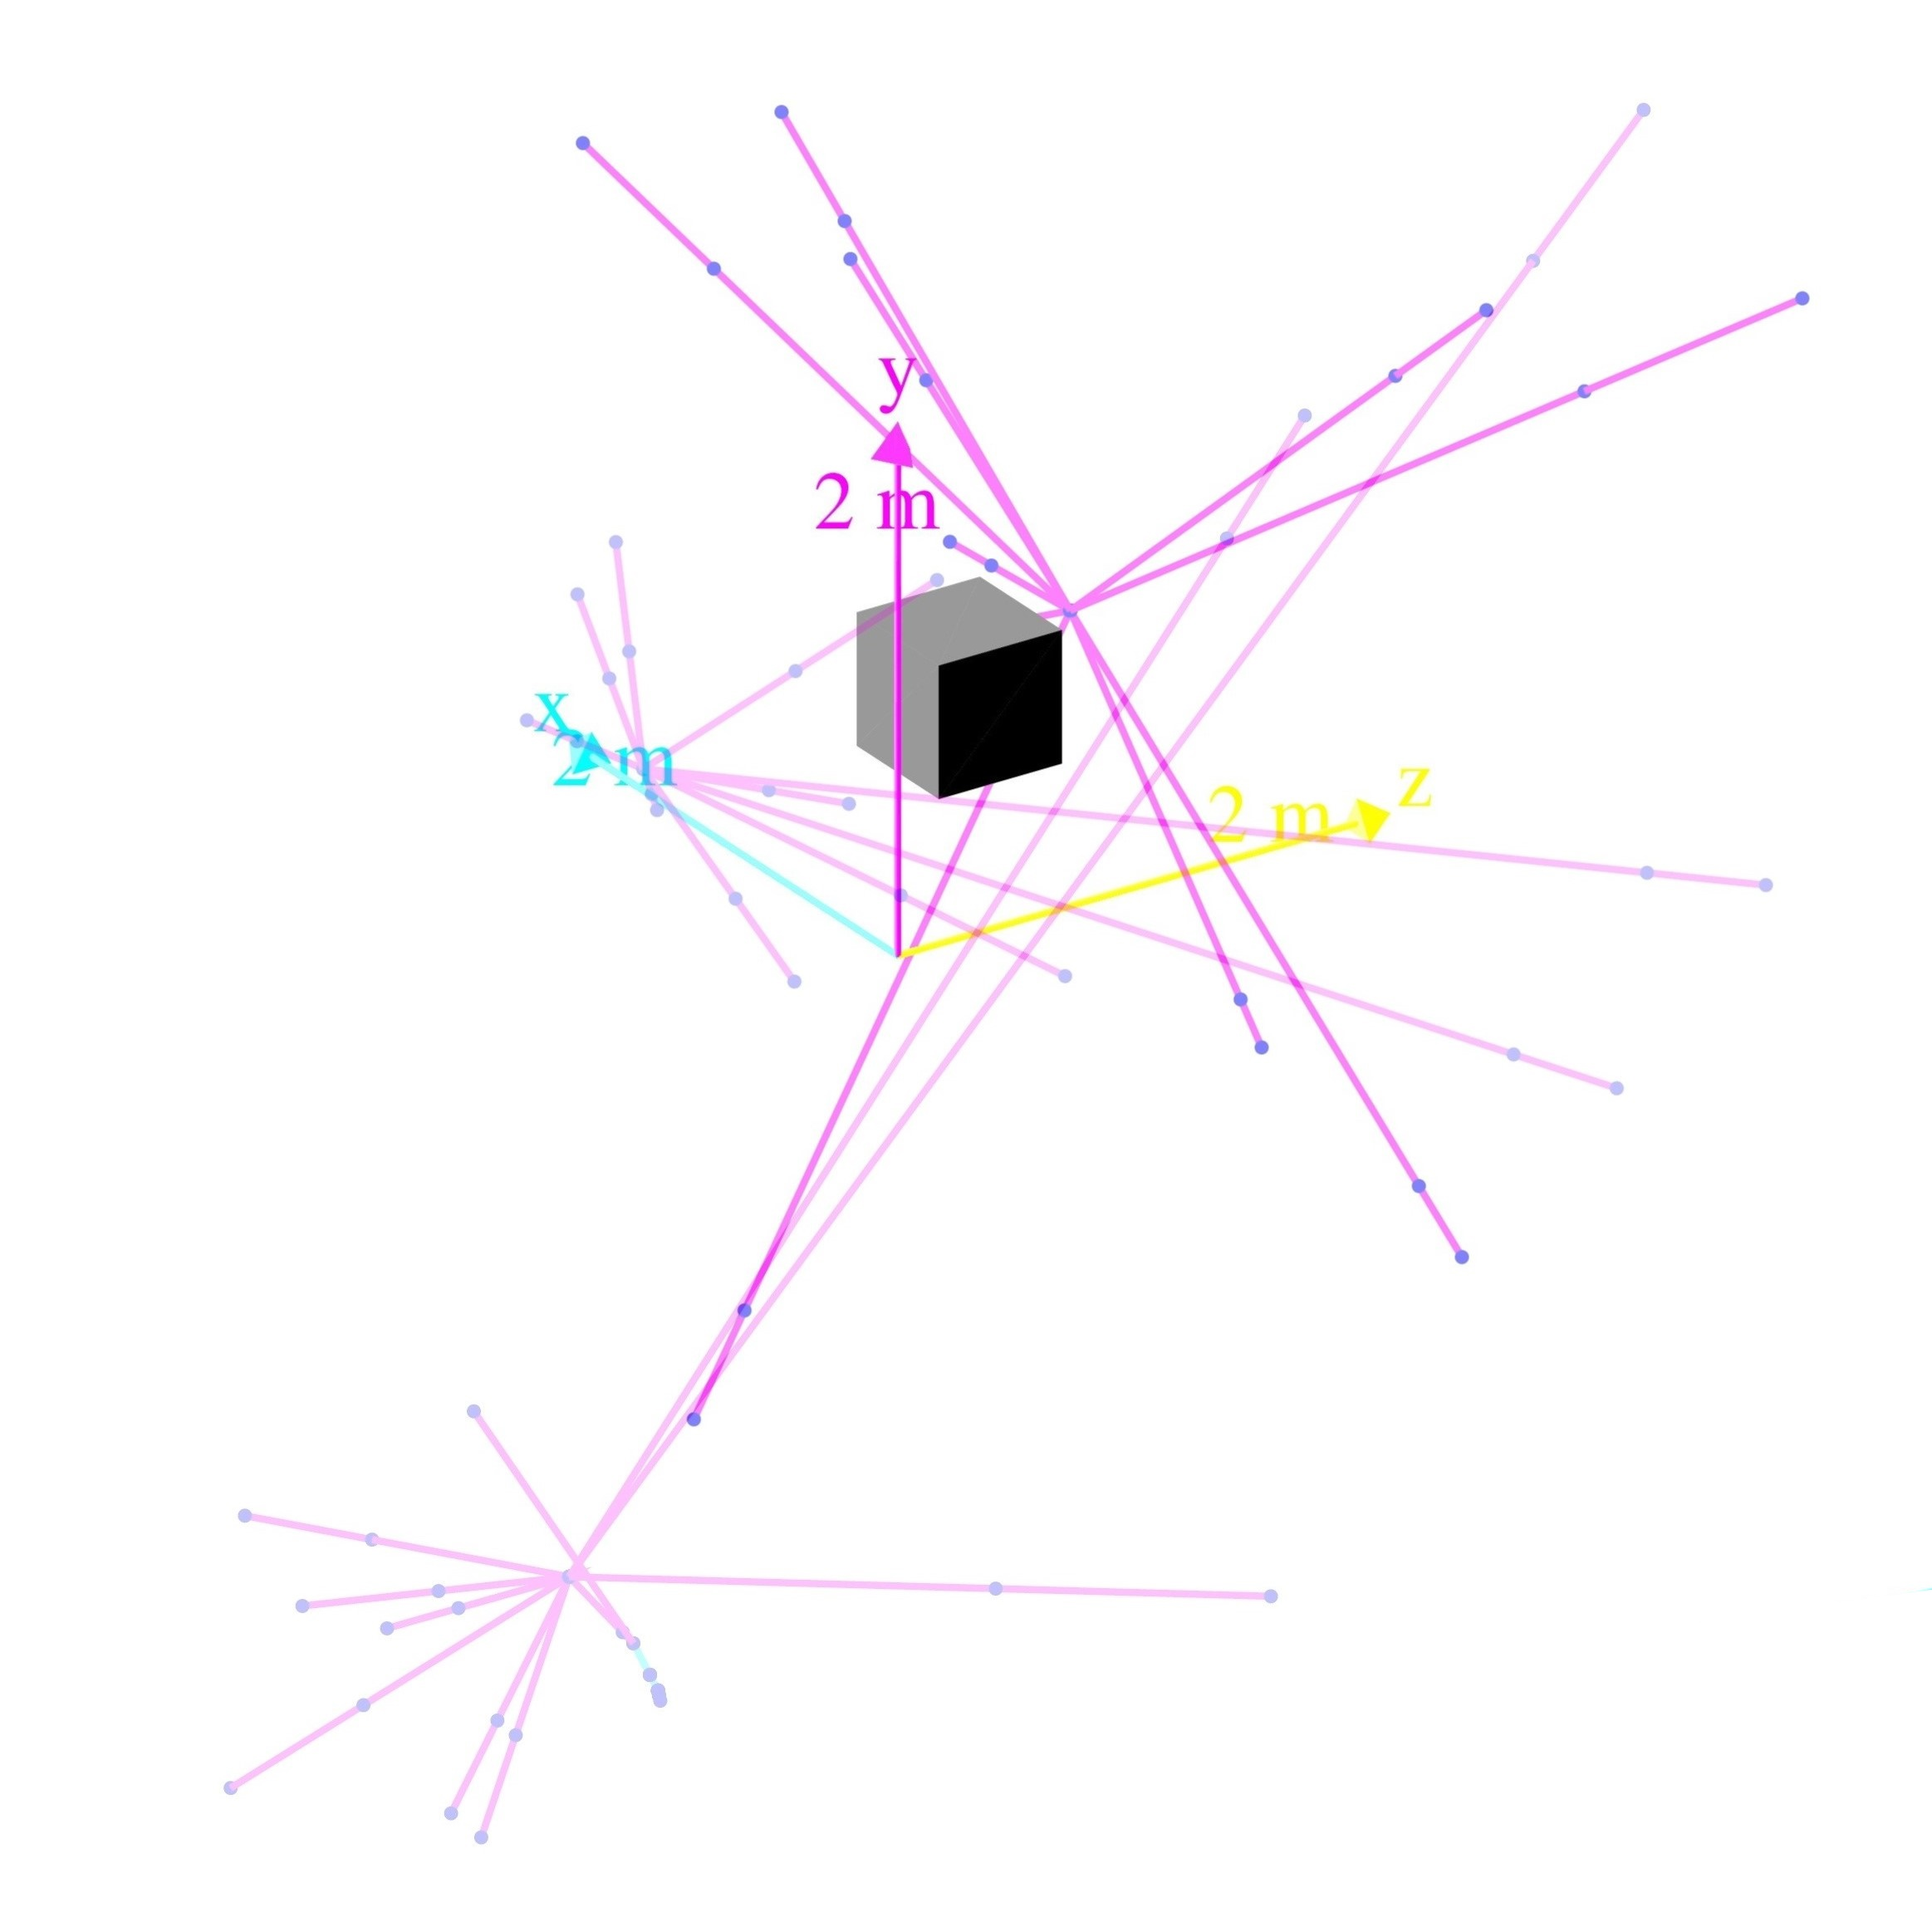
\includegraphics[width=0.24\textwidth]{figures/Geant4/MultiSources.jpg}\label{fig:exph2}}
        \subfigure[多点源有屏蔽]{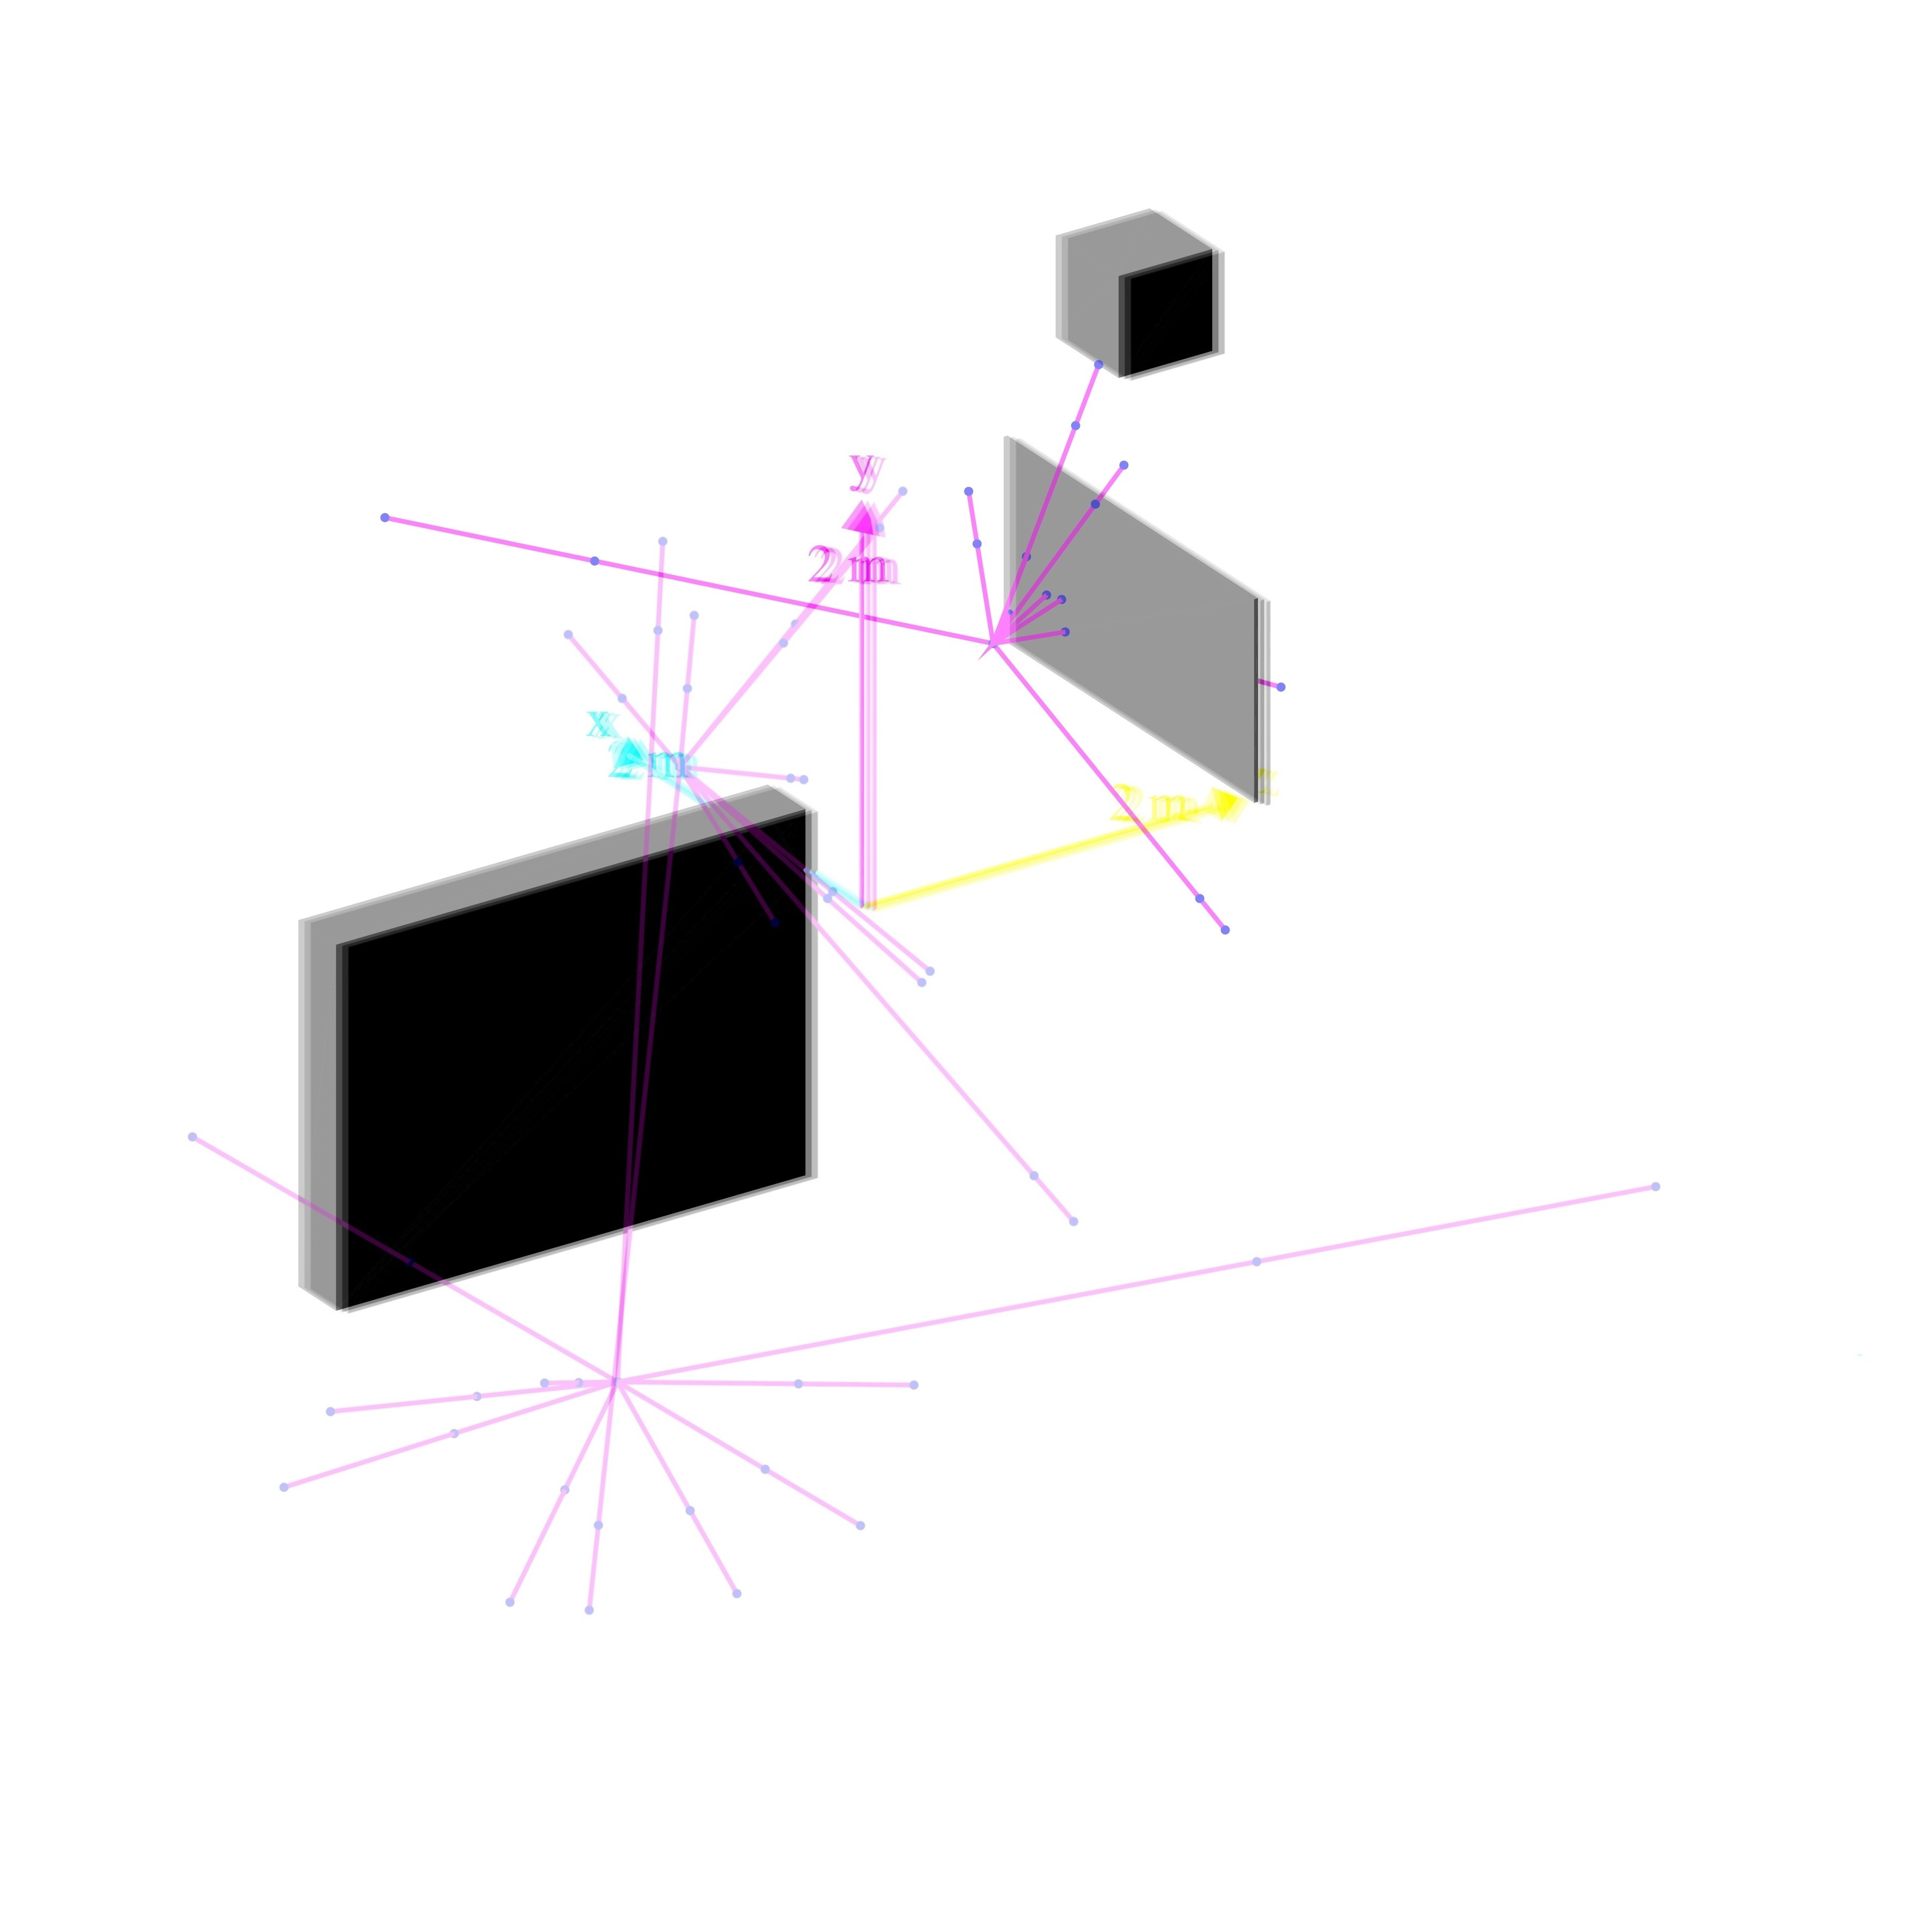
\includegraphics[width=0.24\textwidth]{figures/Geant4/MultiSourcesShield.jpg}\label{fig:exgr2}}
    \end{figure}
\end{frame}

\begin{frame}
    \frametitle{辐射场重构可视化}
    \begin{figure}[htbp]
        \centering
        \subfigure[单点源无屏蔽]{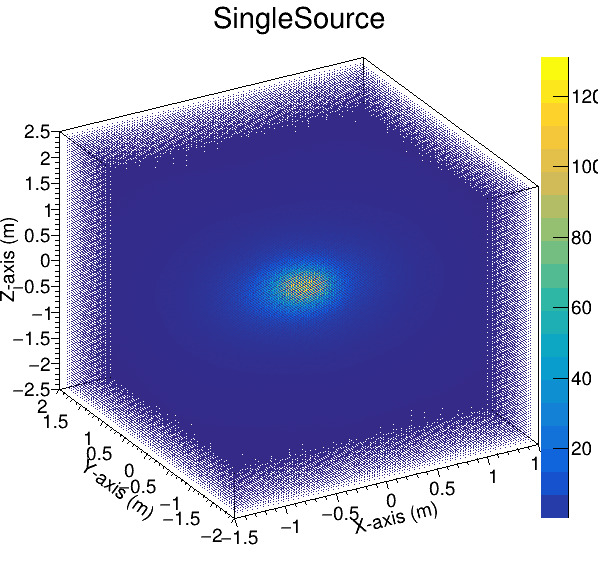
\includegraphics[width=0.25\textwidth]{figures/Vis/SingleSource.png}\label{fig:exph3}}
        \subfigure[单点源有屏蔽]{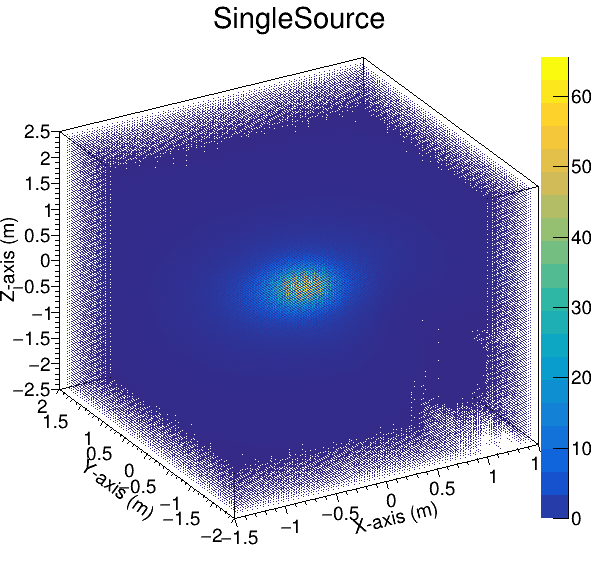
\includegraphics[width=0.25\textwidth]{figures/Vis/SingleSoourceShielded.png}\label{fig:exgr3}}

        \subfigure[多点源无屏蔽]{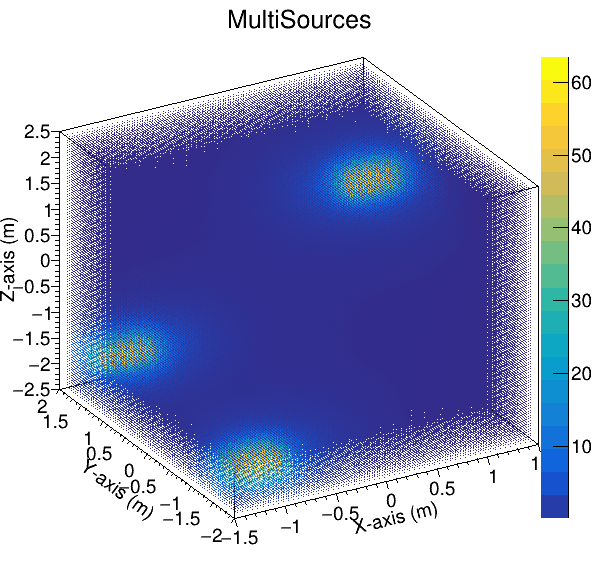
\includegraphics[width=0.25\textwidth]{figures/Vis/MultiSources.png}\label{fig:exph4}}
        \subfigure[多点源有屏蔽]{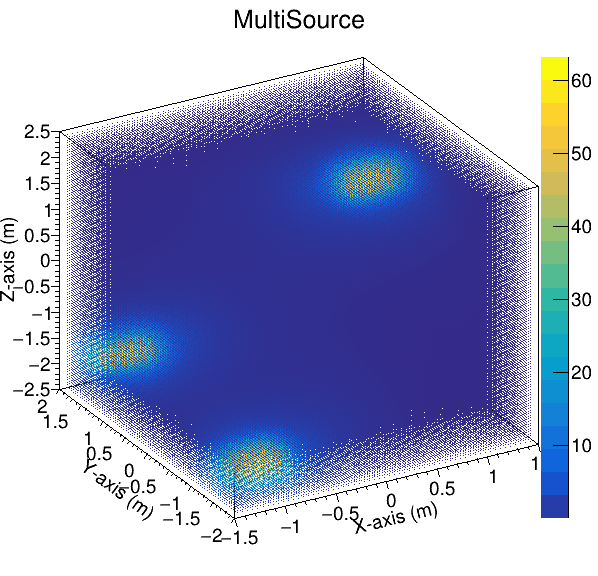
\includegraphics[width=0.25\textwidth]{figures/Vis/MultiSourcesShielded.png}\label{fig:exgr4}}
    \end{figure}
\end{frame}

\begin{frame}
    \frametitle{辐射场重构偏差}
    \begin{figure}[htbp]
        \centering
        \subfigure[$ \sigma = 0.19 $]{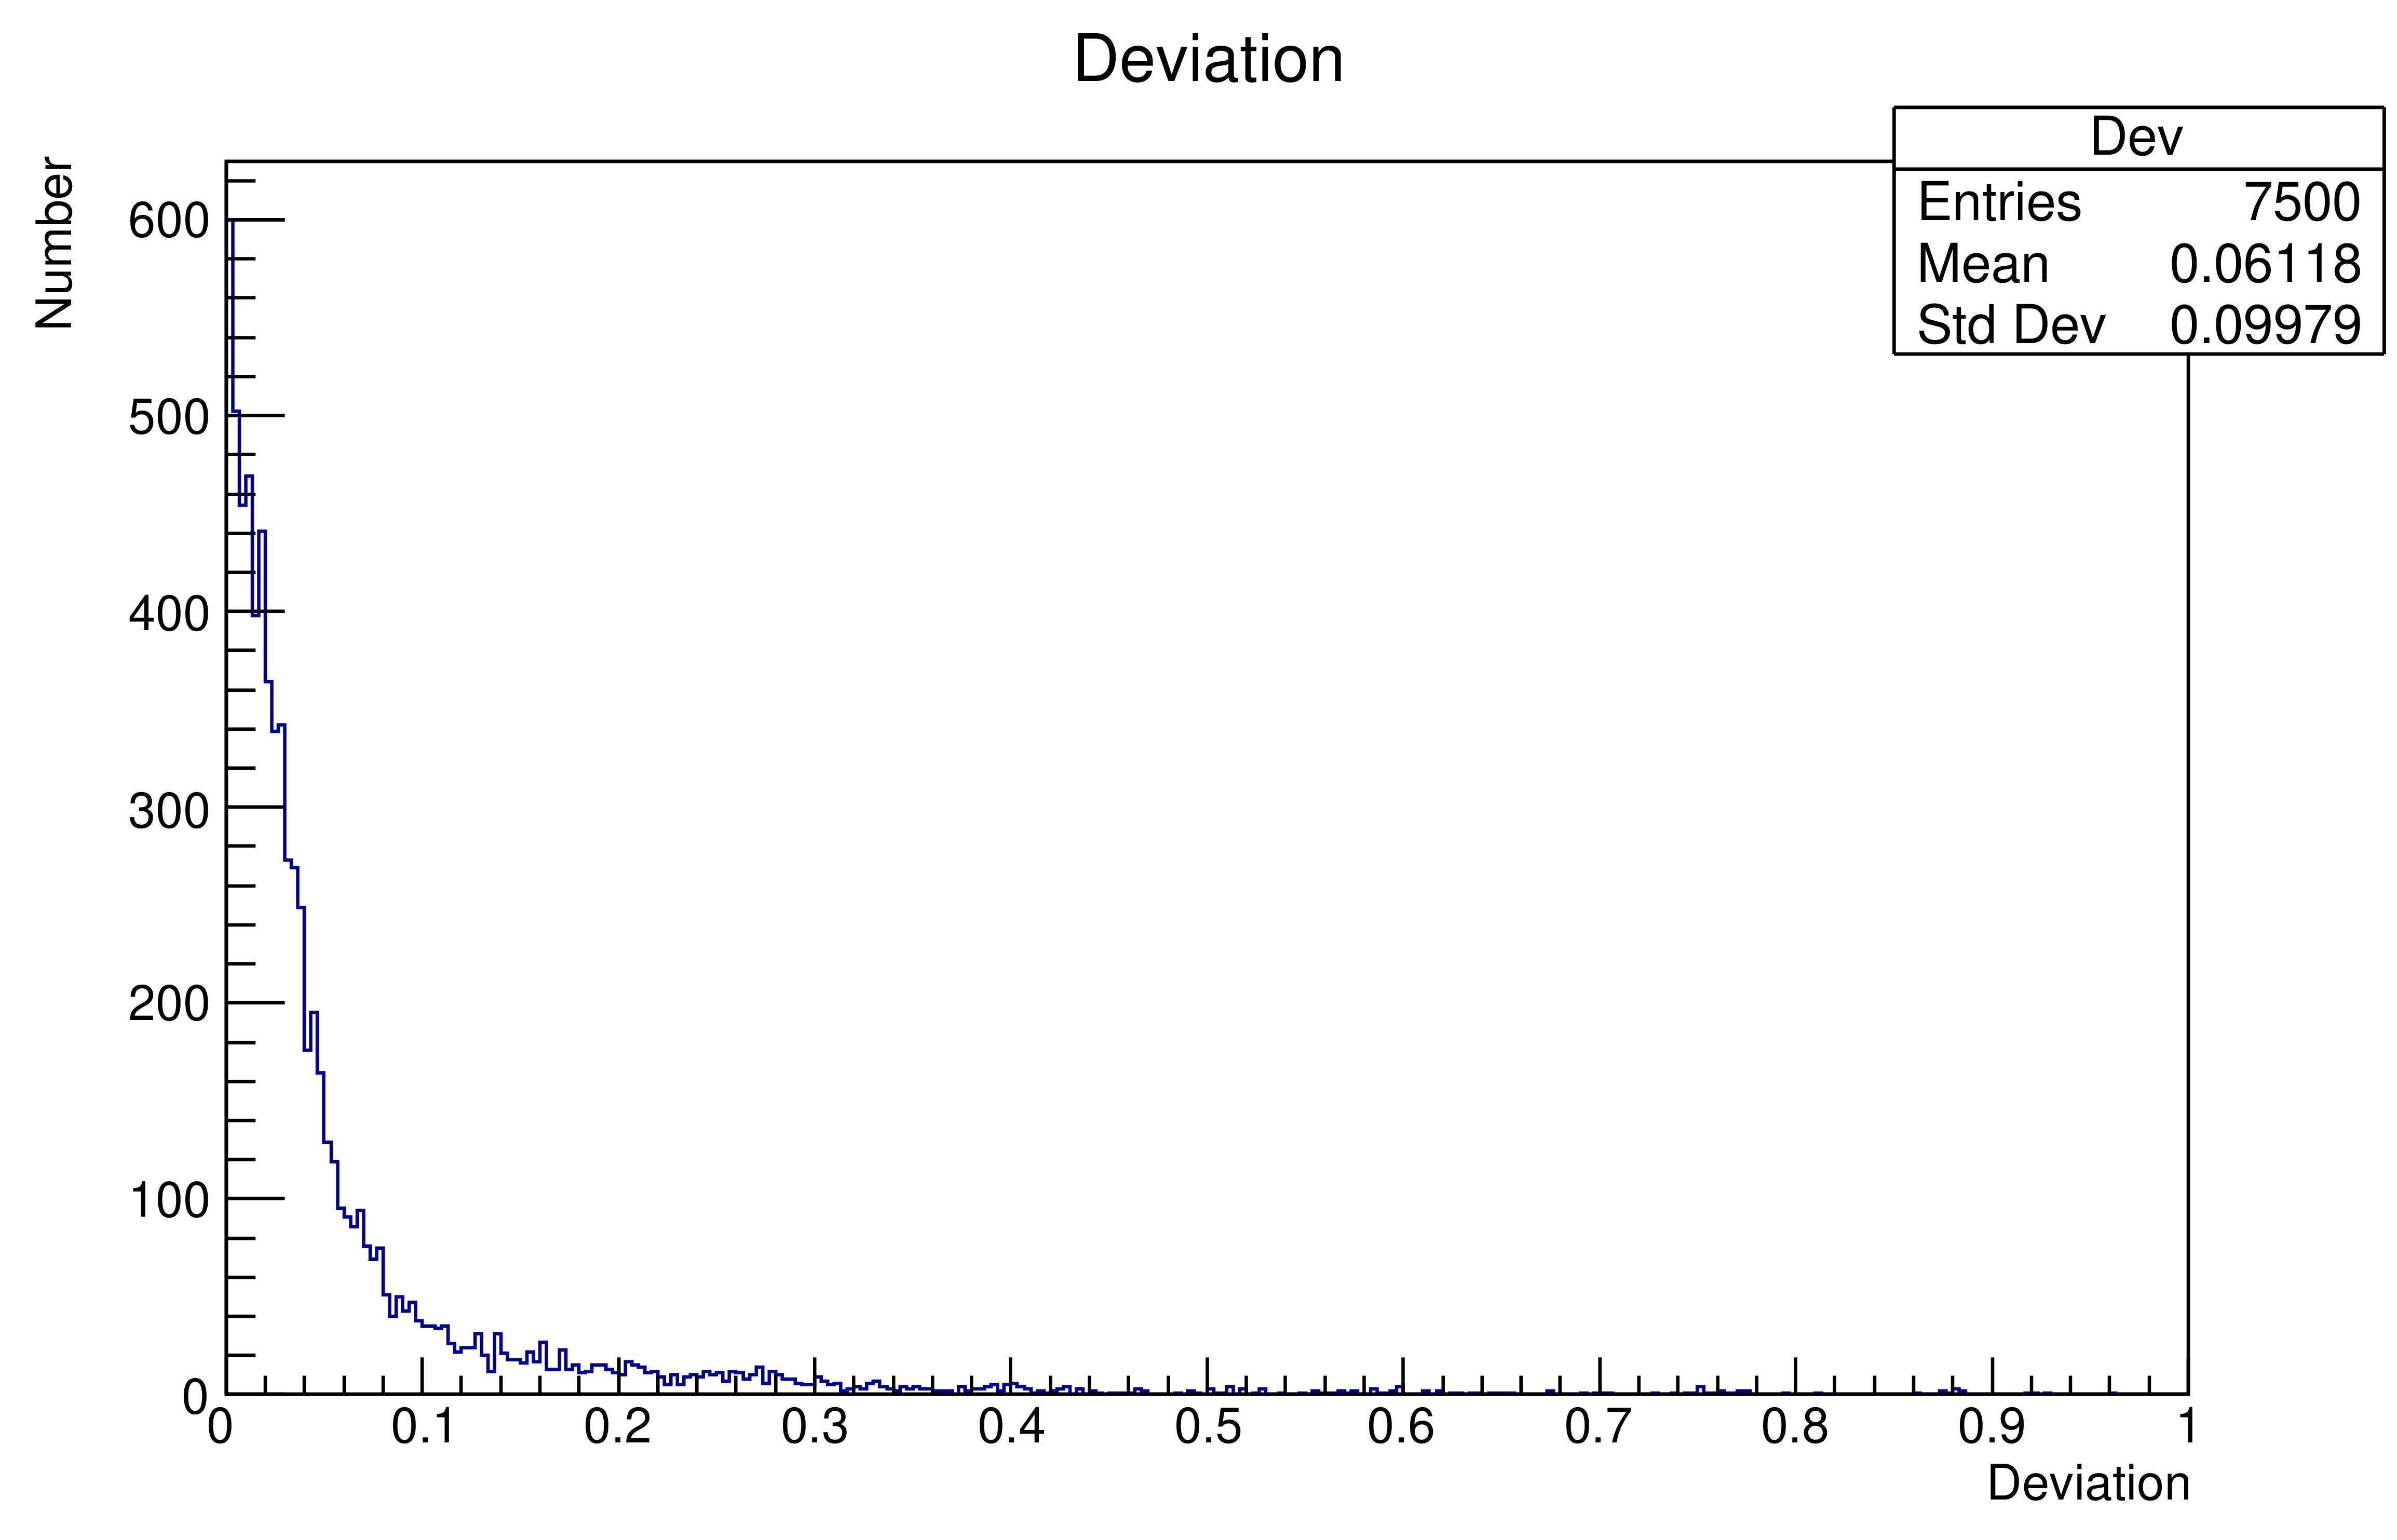
\includegraphics[width=0.25\textwidth]{figures/Deviation/Innvation/SingleSourceUnshield.jpg}\label{fig:exph5}}
        \subfigure[$ \sigma = 0.45 $]{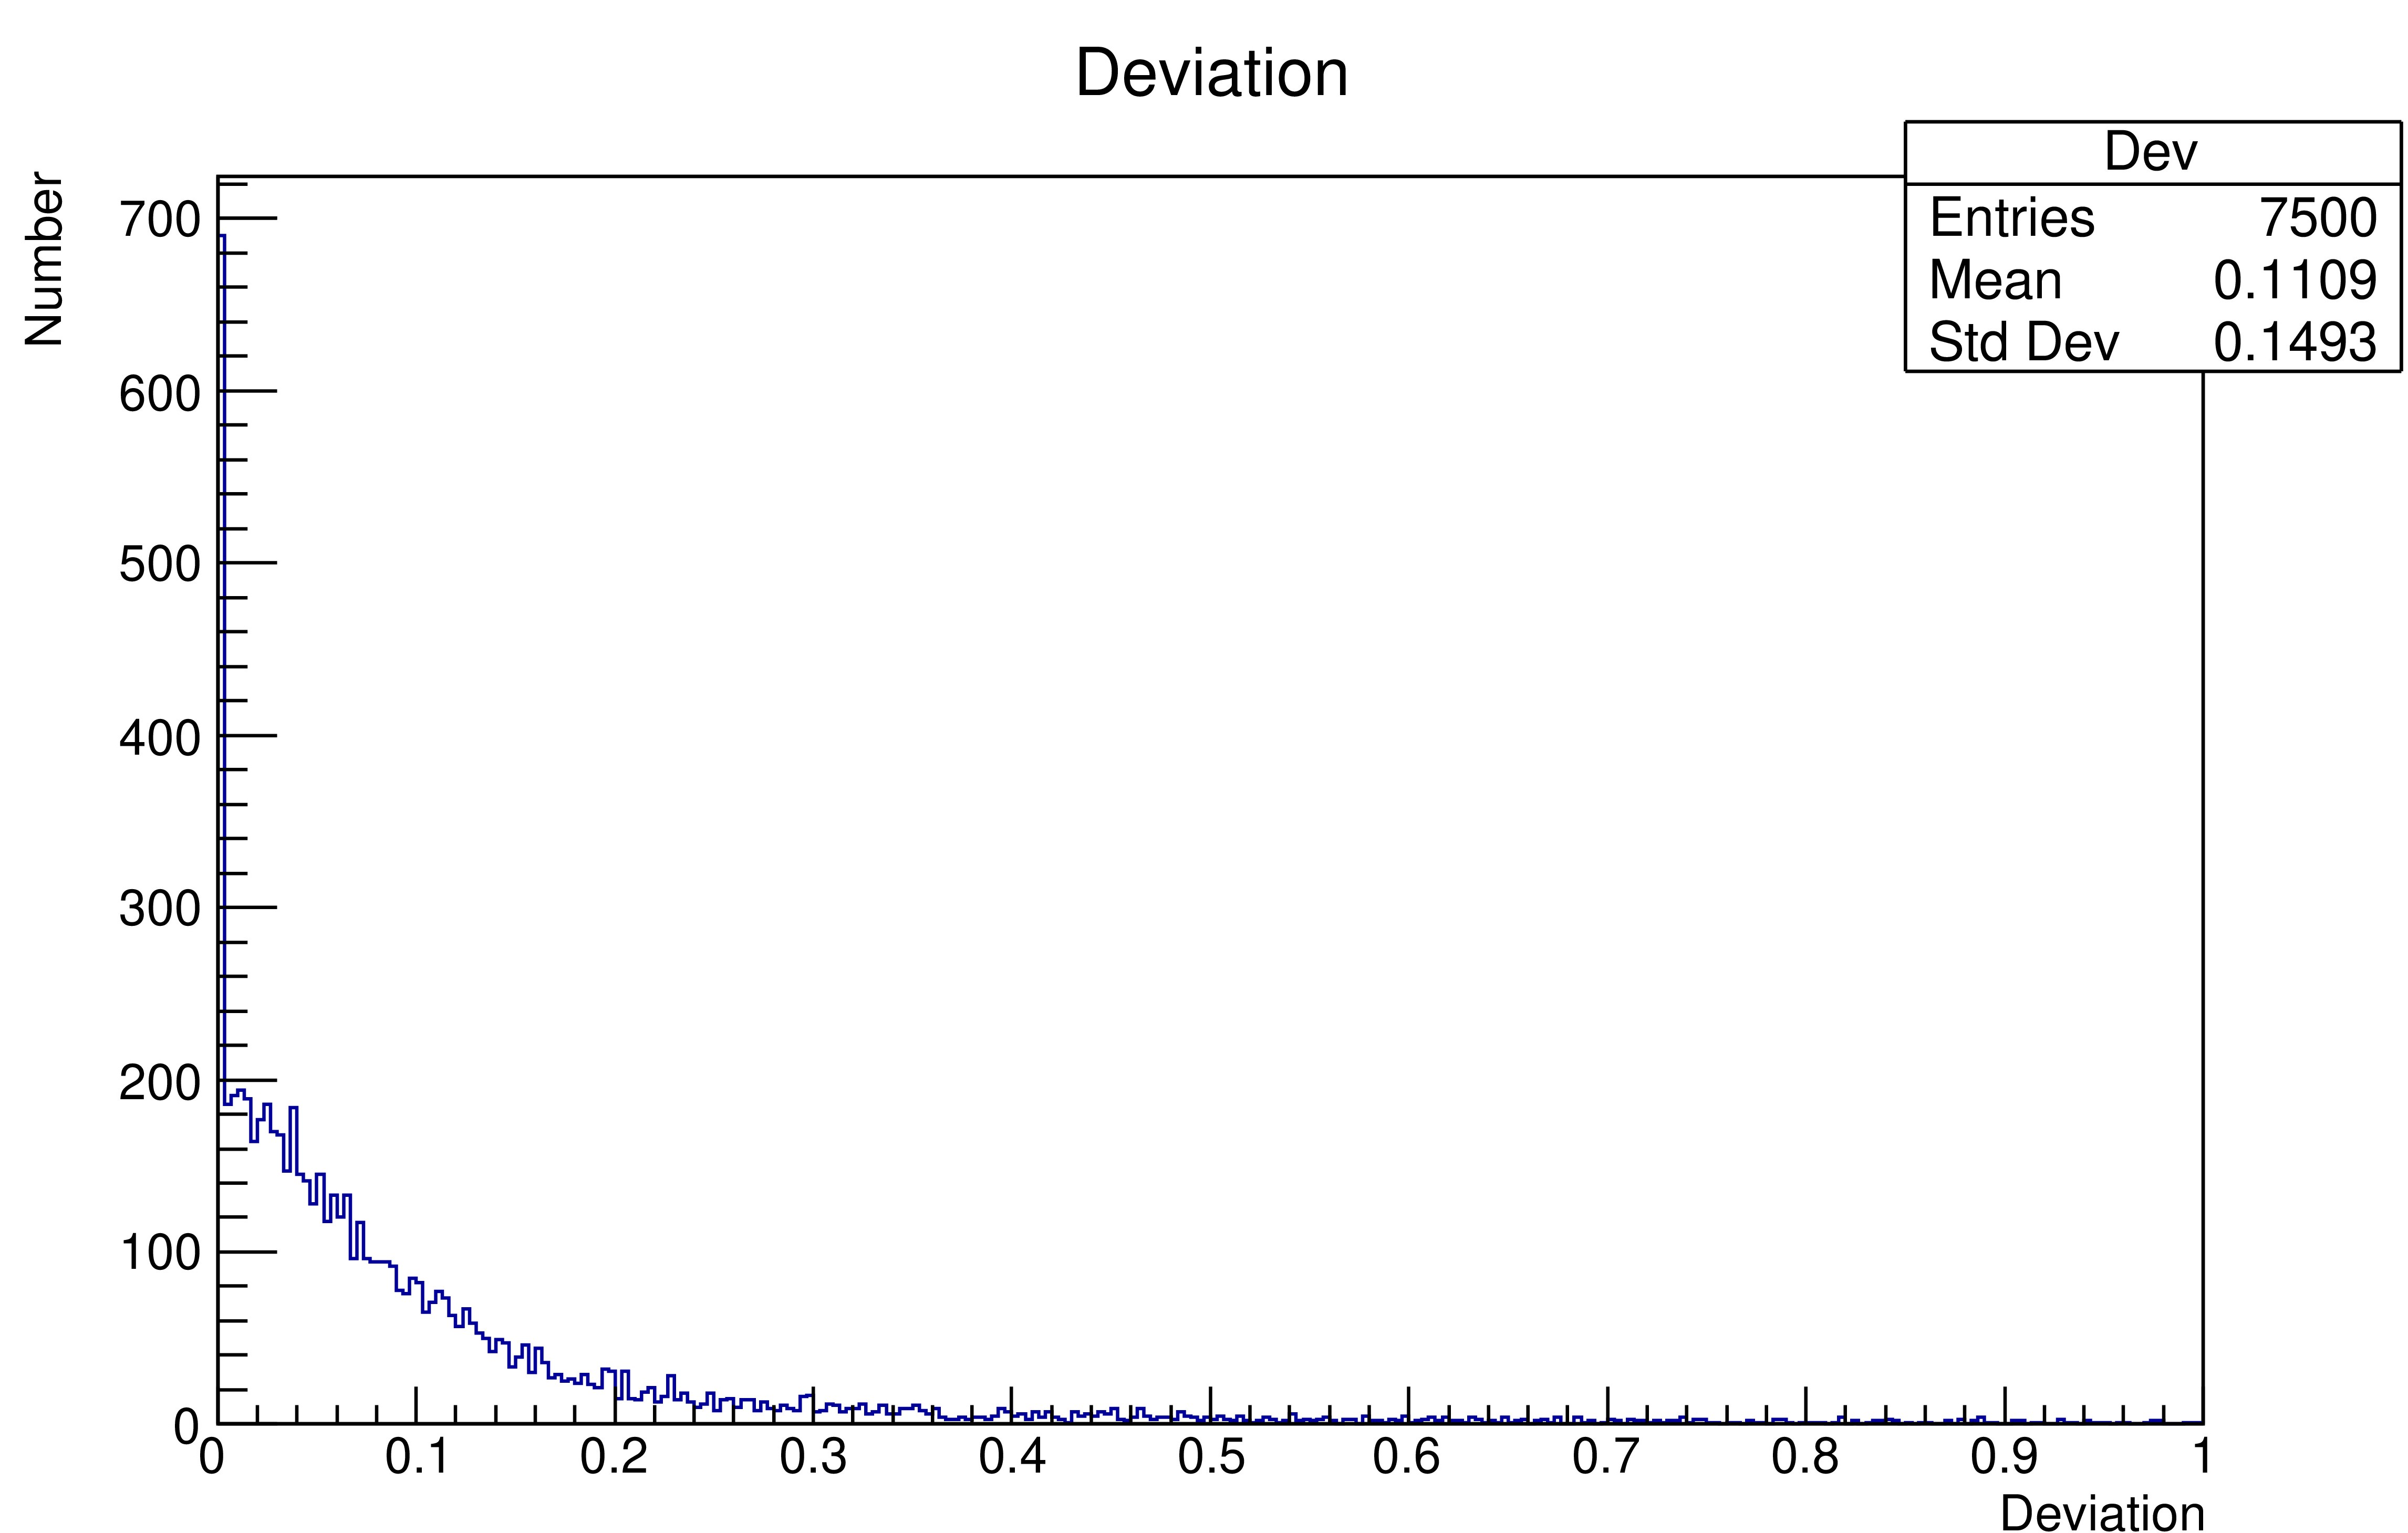
\includegraphics[width=0.25\textwidth]{figures/Deviation/Innvation/SingleSourceShield.jpg}\label{fig:exgr5}}

        \subfigure[$ \sigma = 0.37 $]{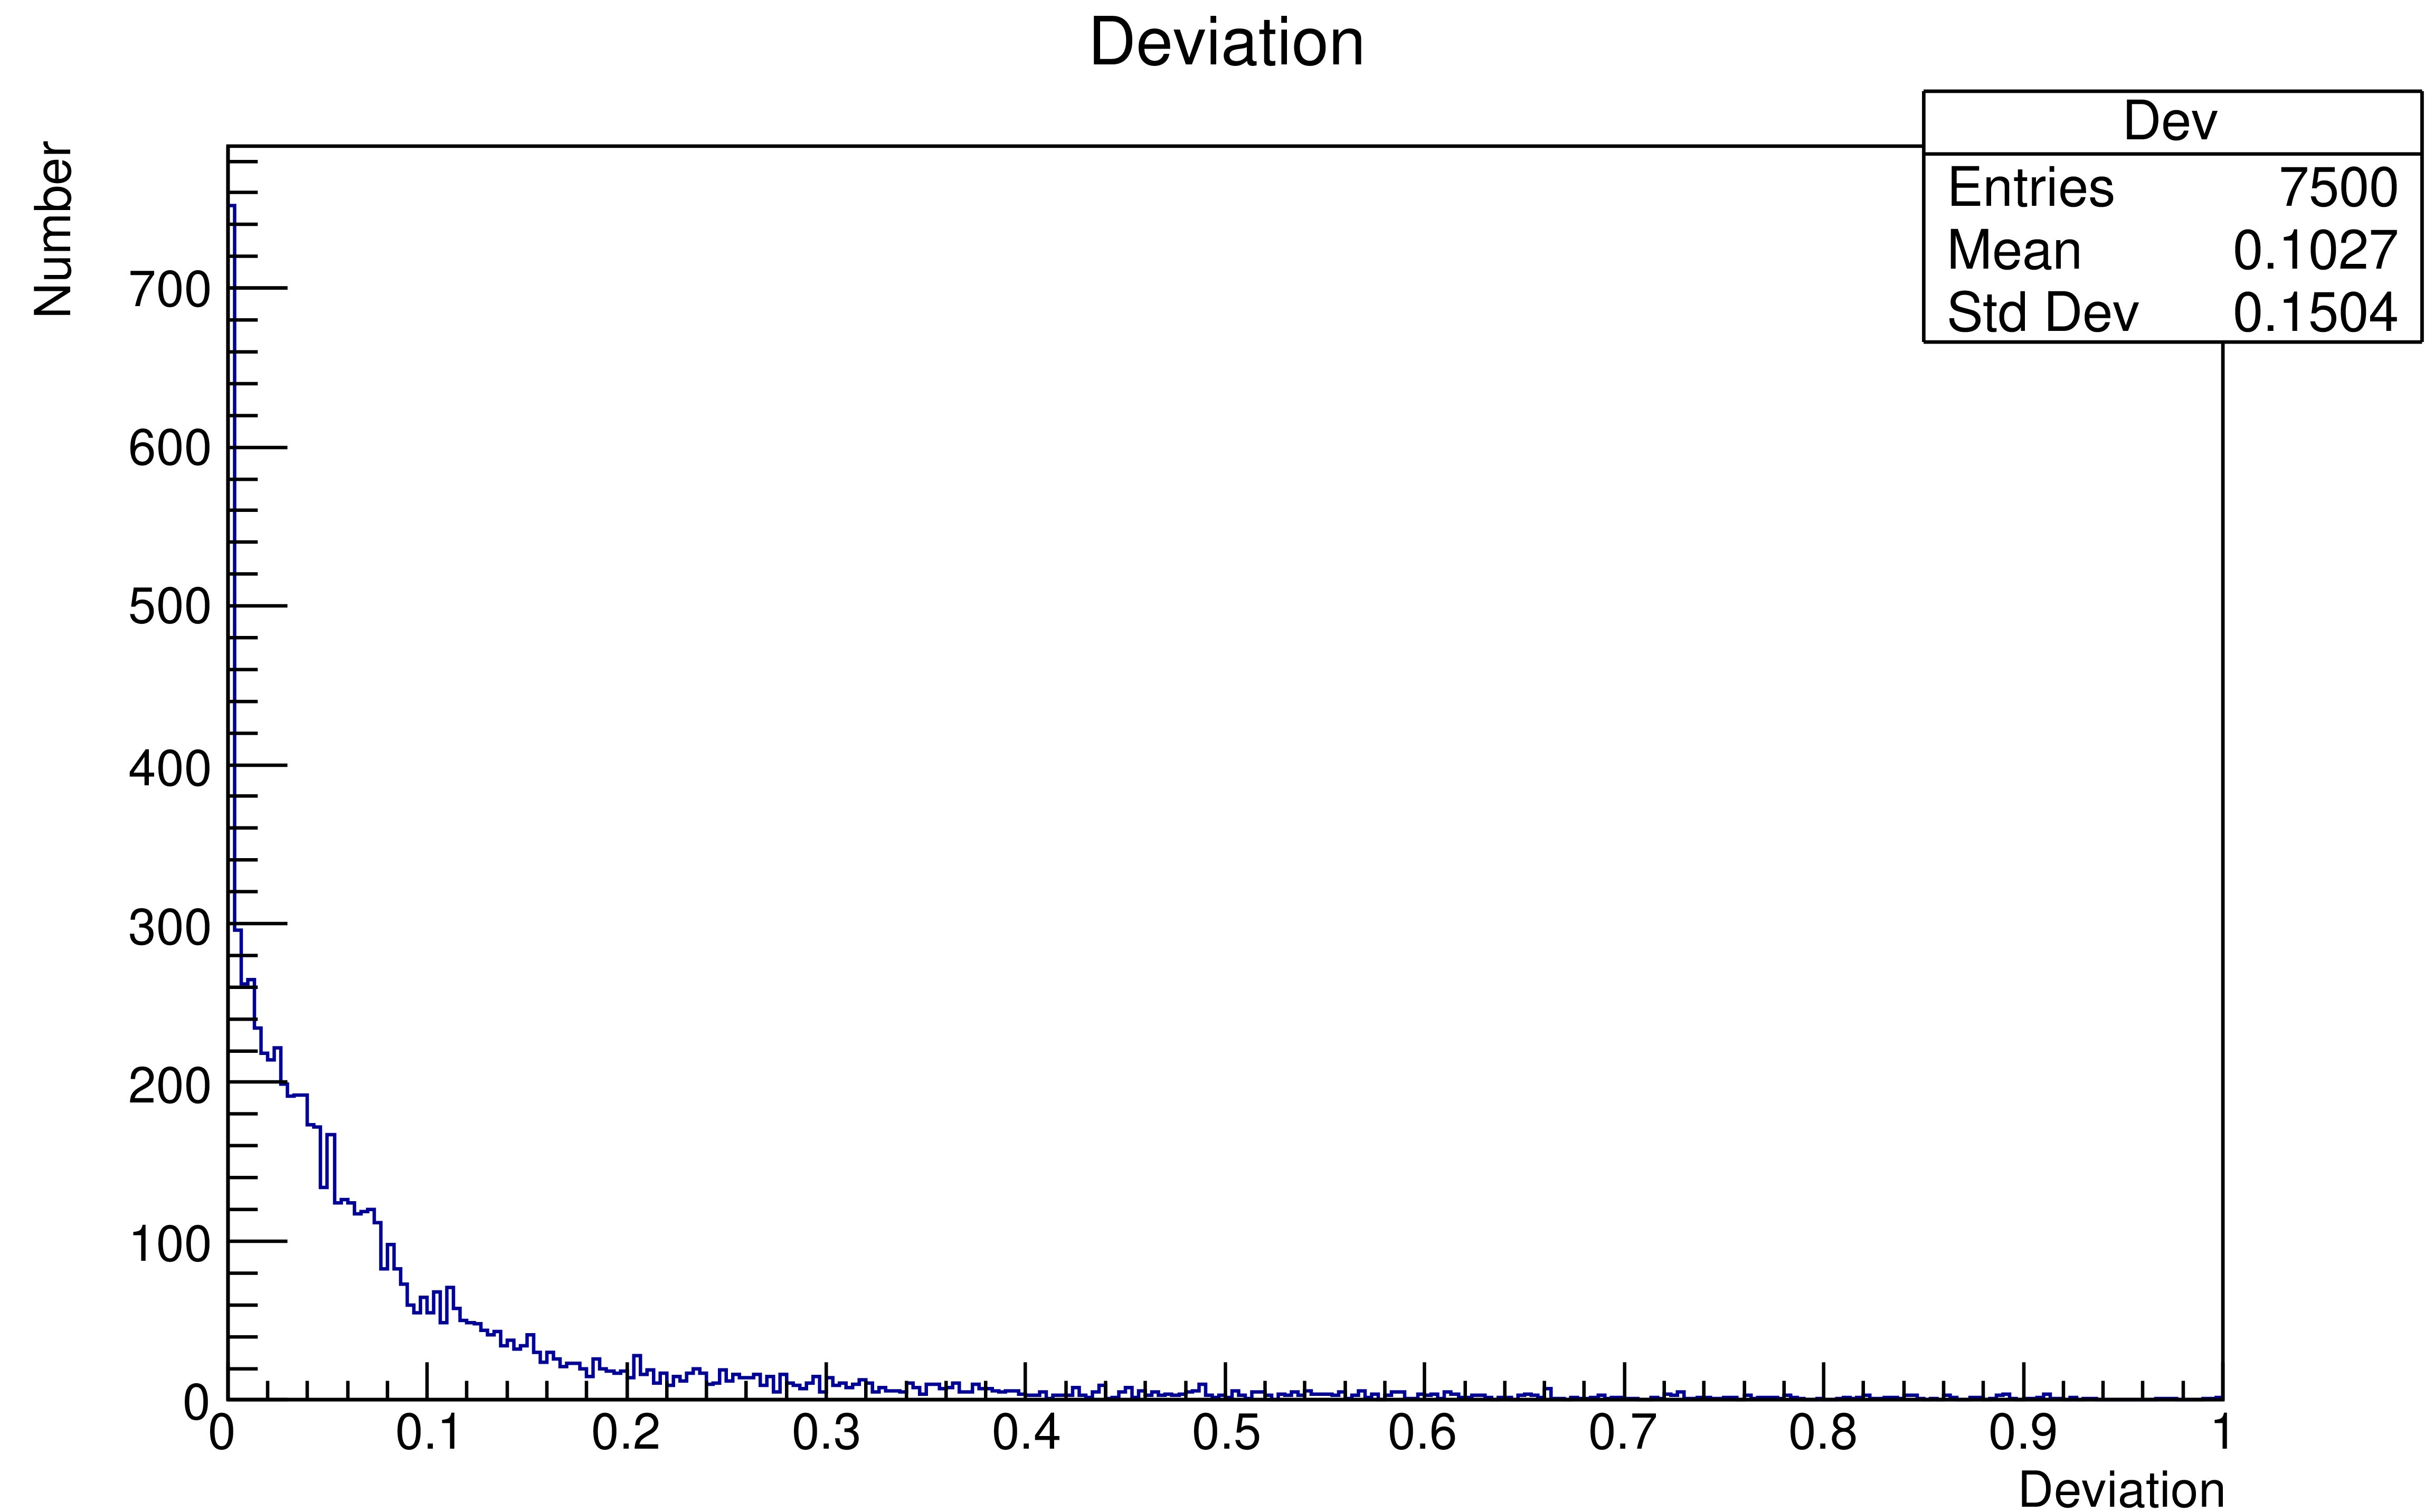
\includegraphics[width=0.25\textwidth]{figures/Deviation/Innvation/MultiSourcesUnshield.jpg}\label{fig:exph6}}
        \subfigure[$ \sigma = 0.55 $]{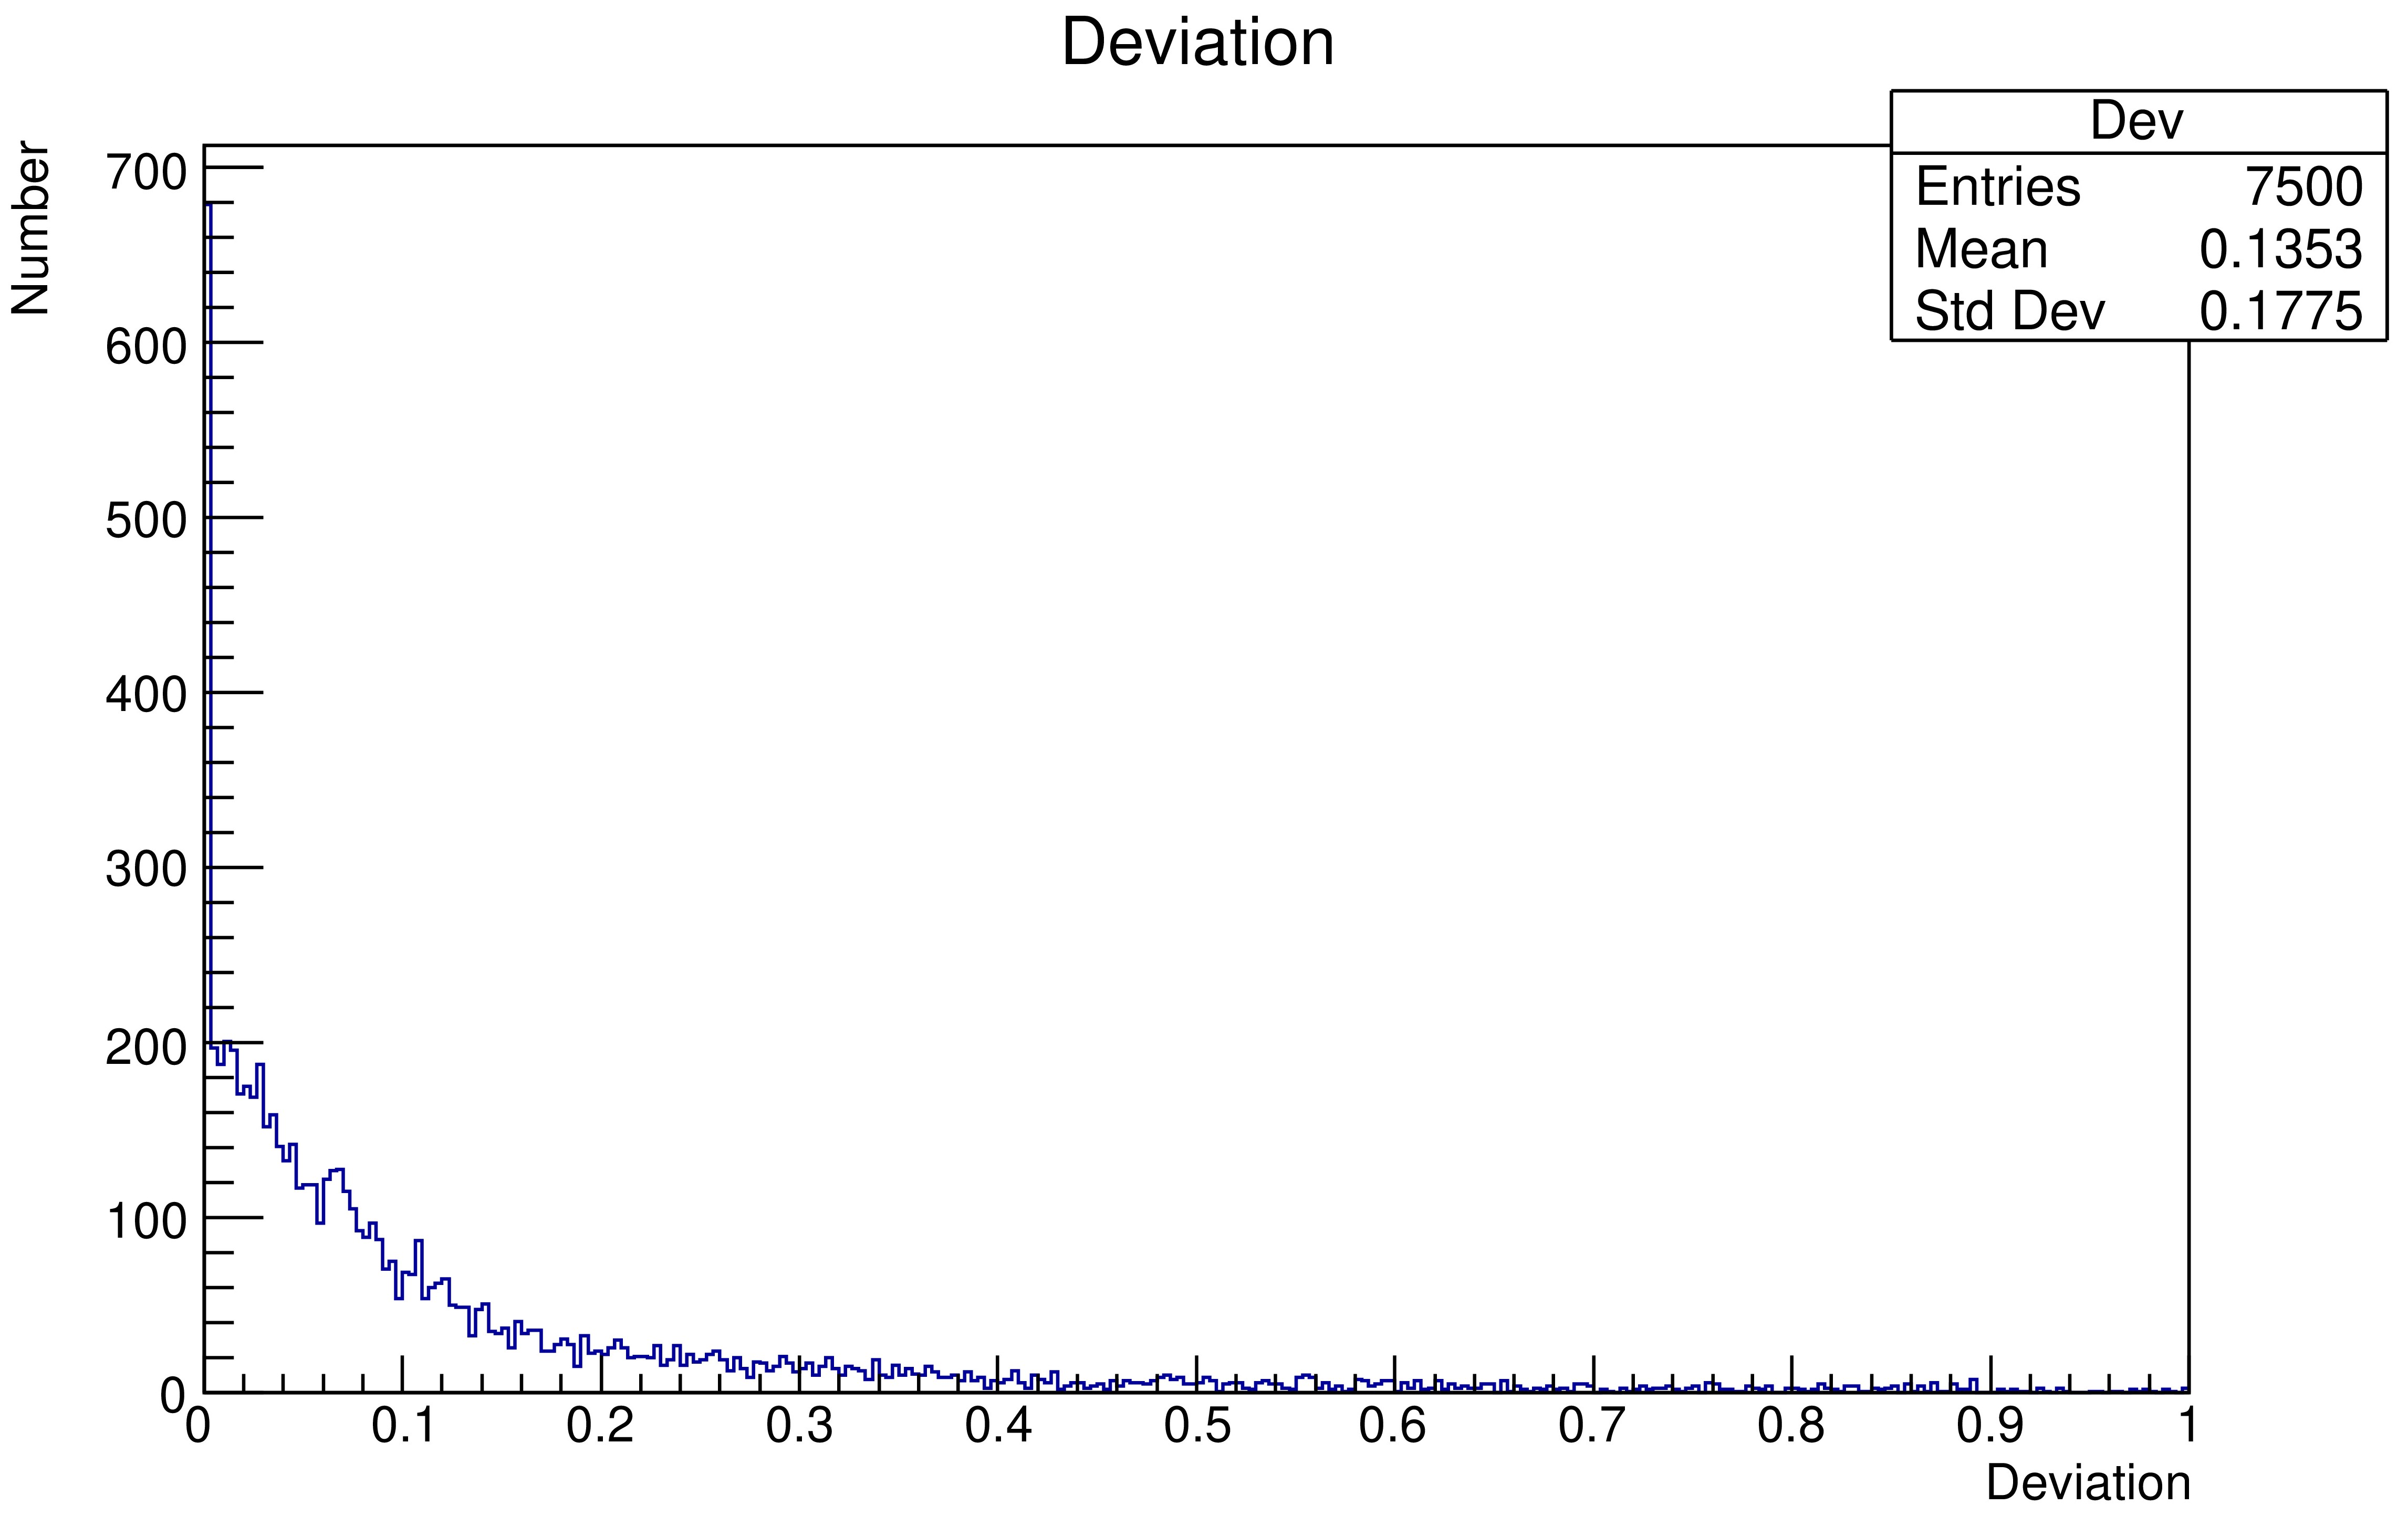
\includegraphics[width=0.25\textwidth]{figures/Deviation/Innvation/MultiSourcesShield.jpg}\label{fig:exgr6}}
    \end{figure}
\end{frame}

\subsection{辐射场重构方法比较}
\begin{frame}
    \frametitle{相对偏差比较}
    \begin{figure}[htbp]
        \centering
        \subfigure[多层B样条插值]{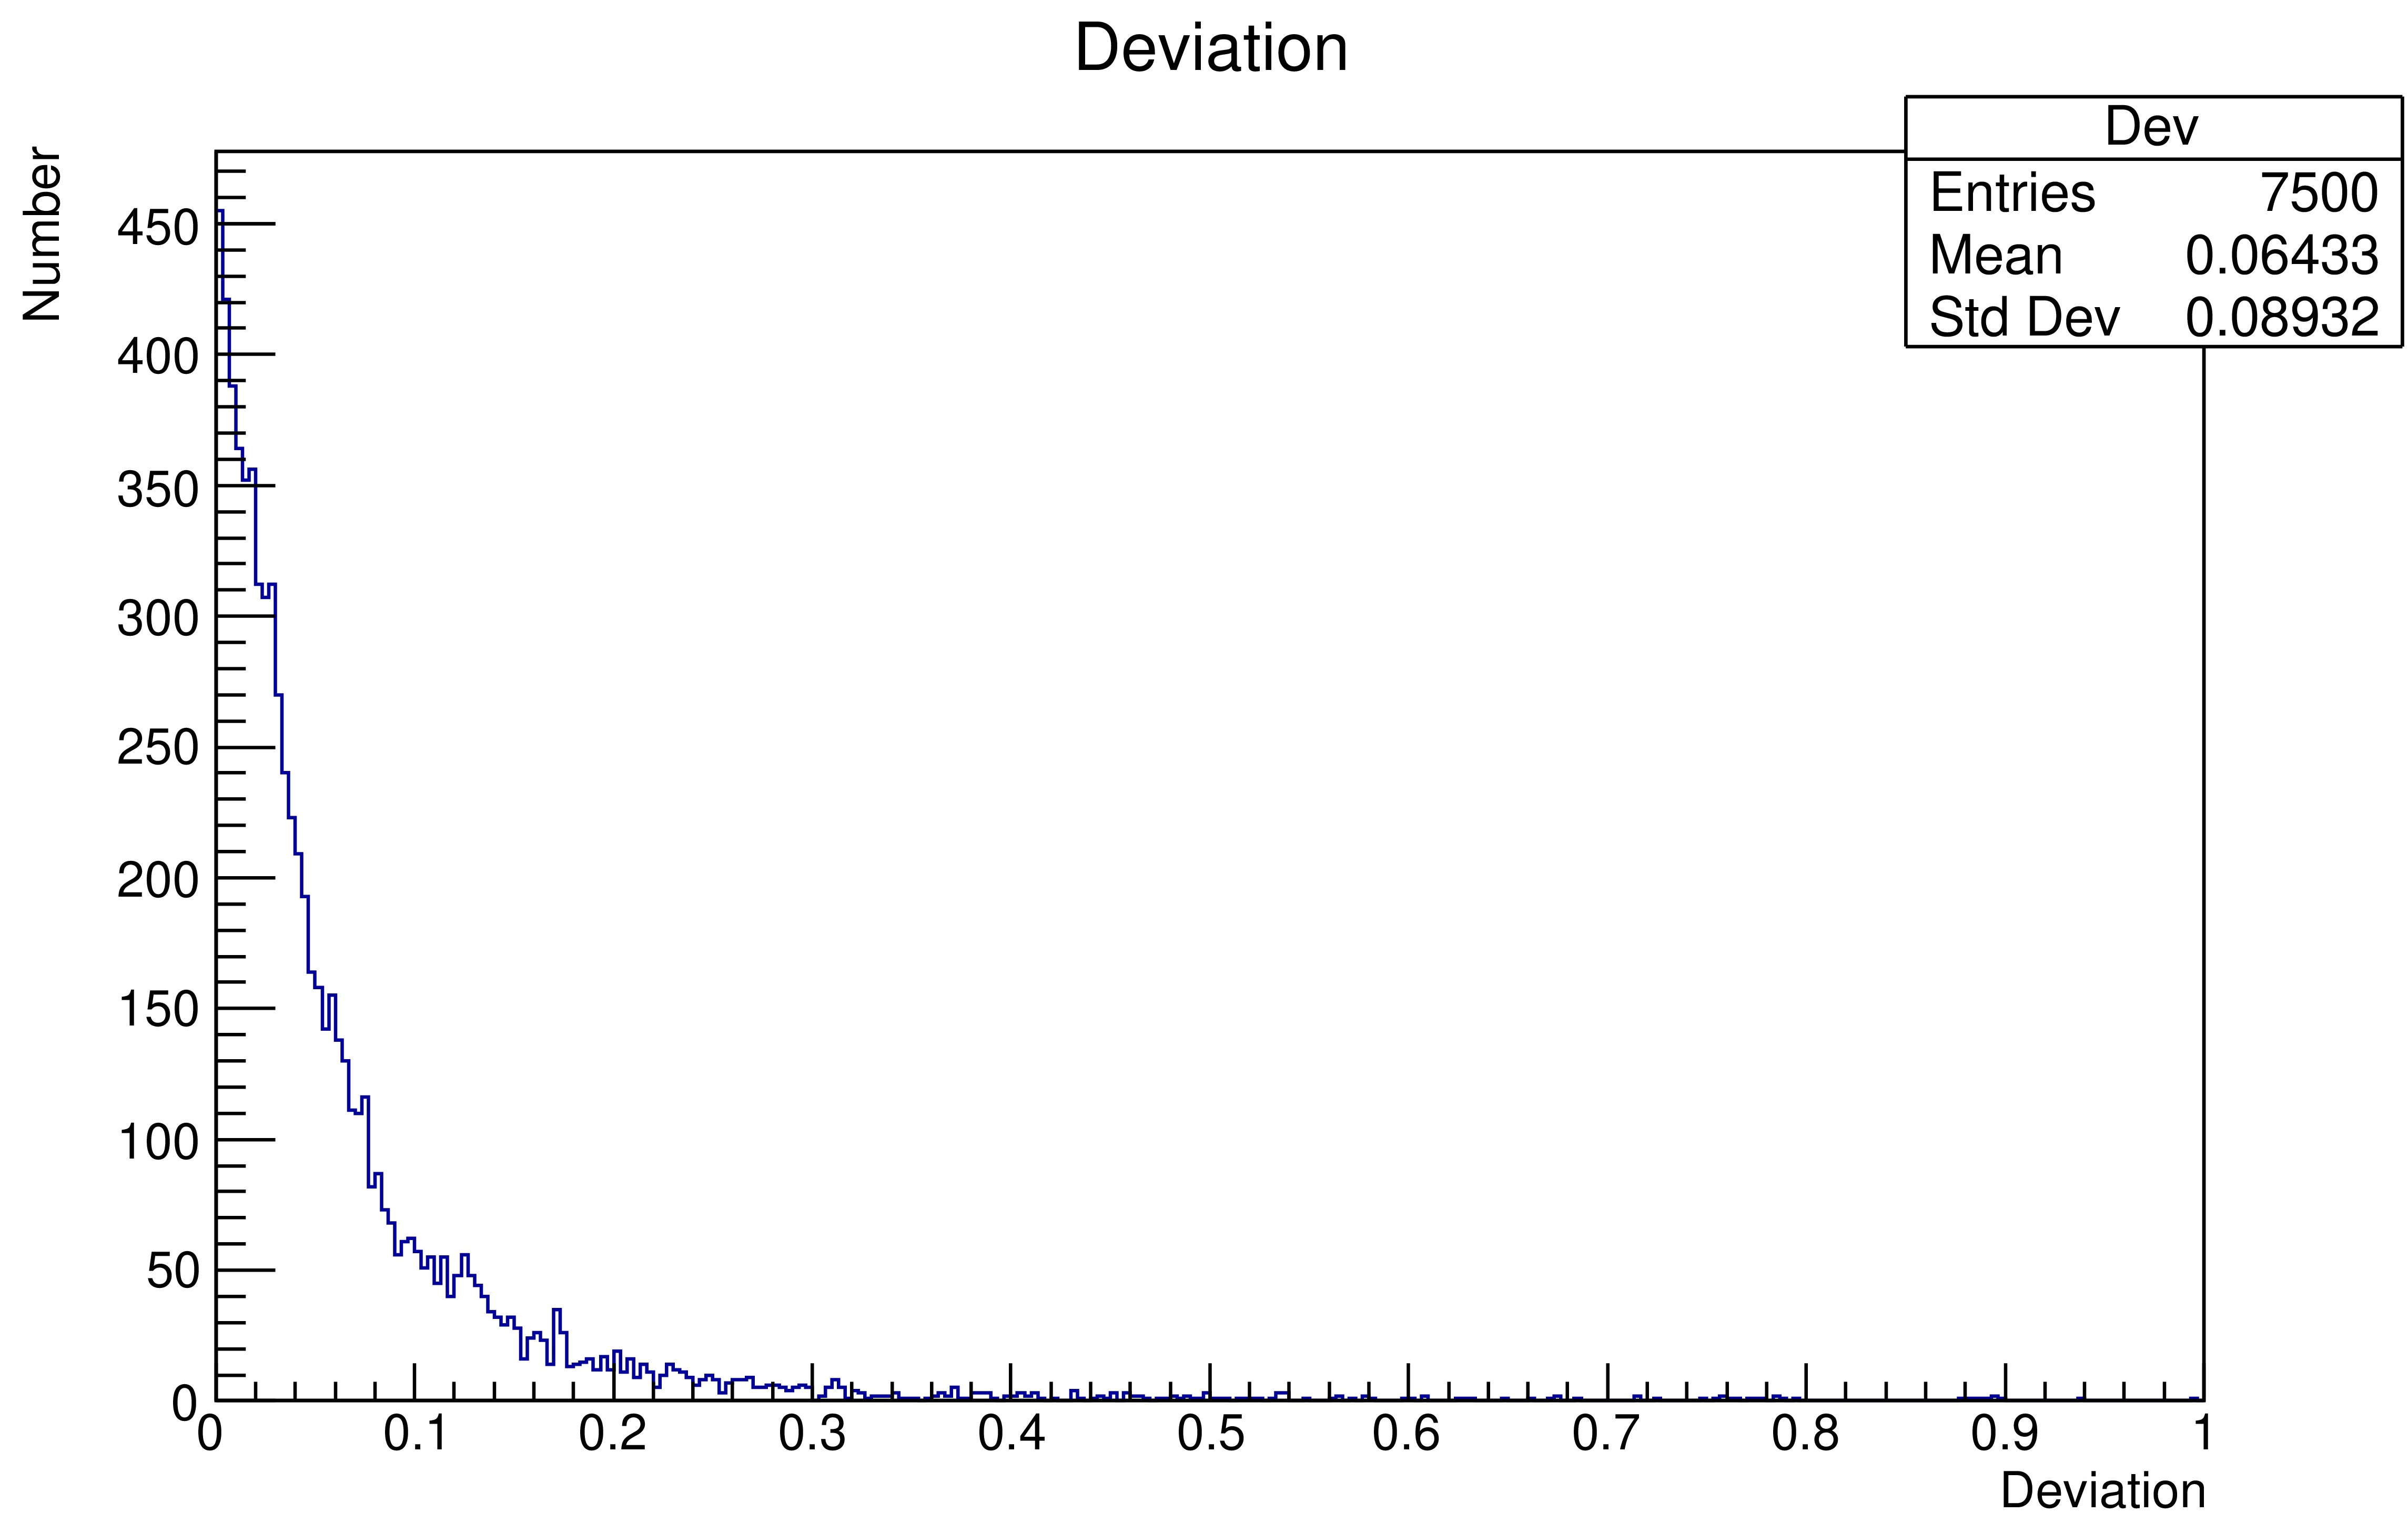
\includegraphics[width=0.45\textwidth]{figures/RD/MBA.jpg}\label{fig:exph7}}
        \subfigure[克里金插值]{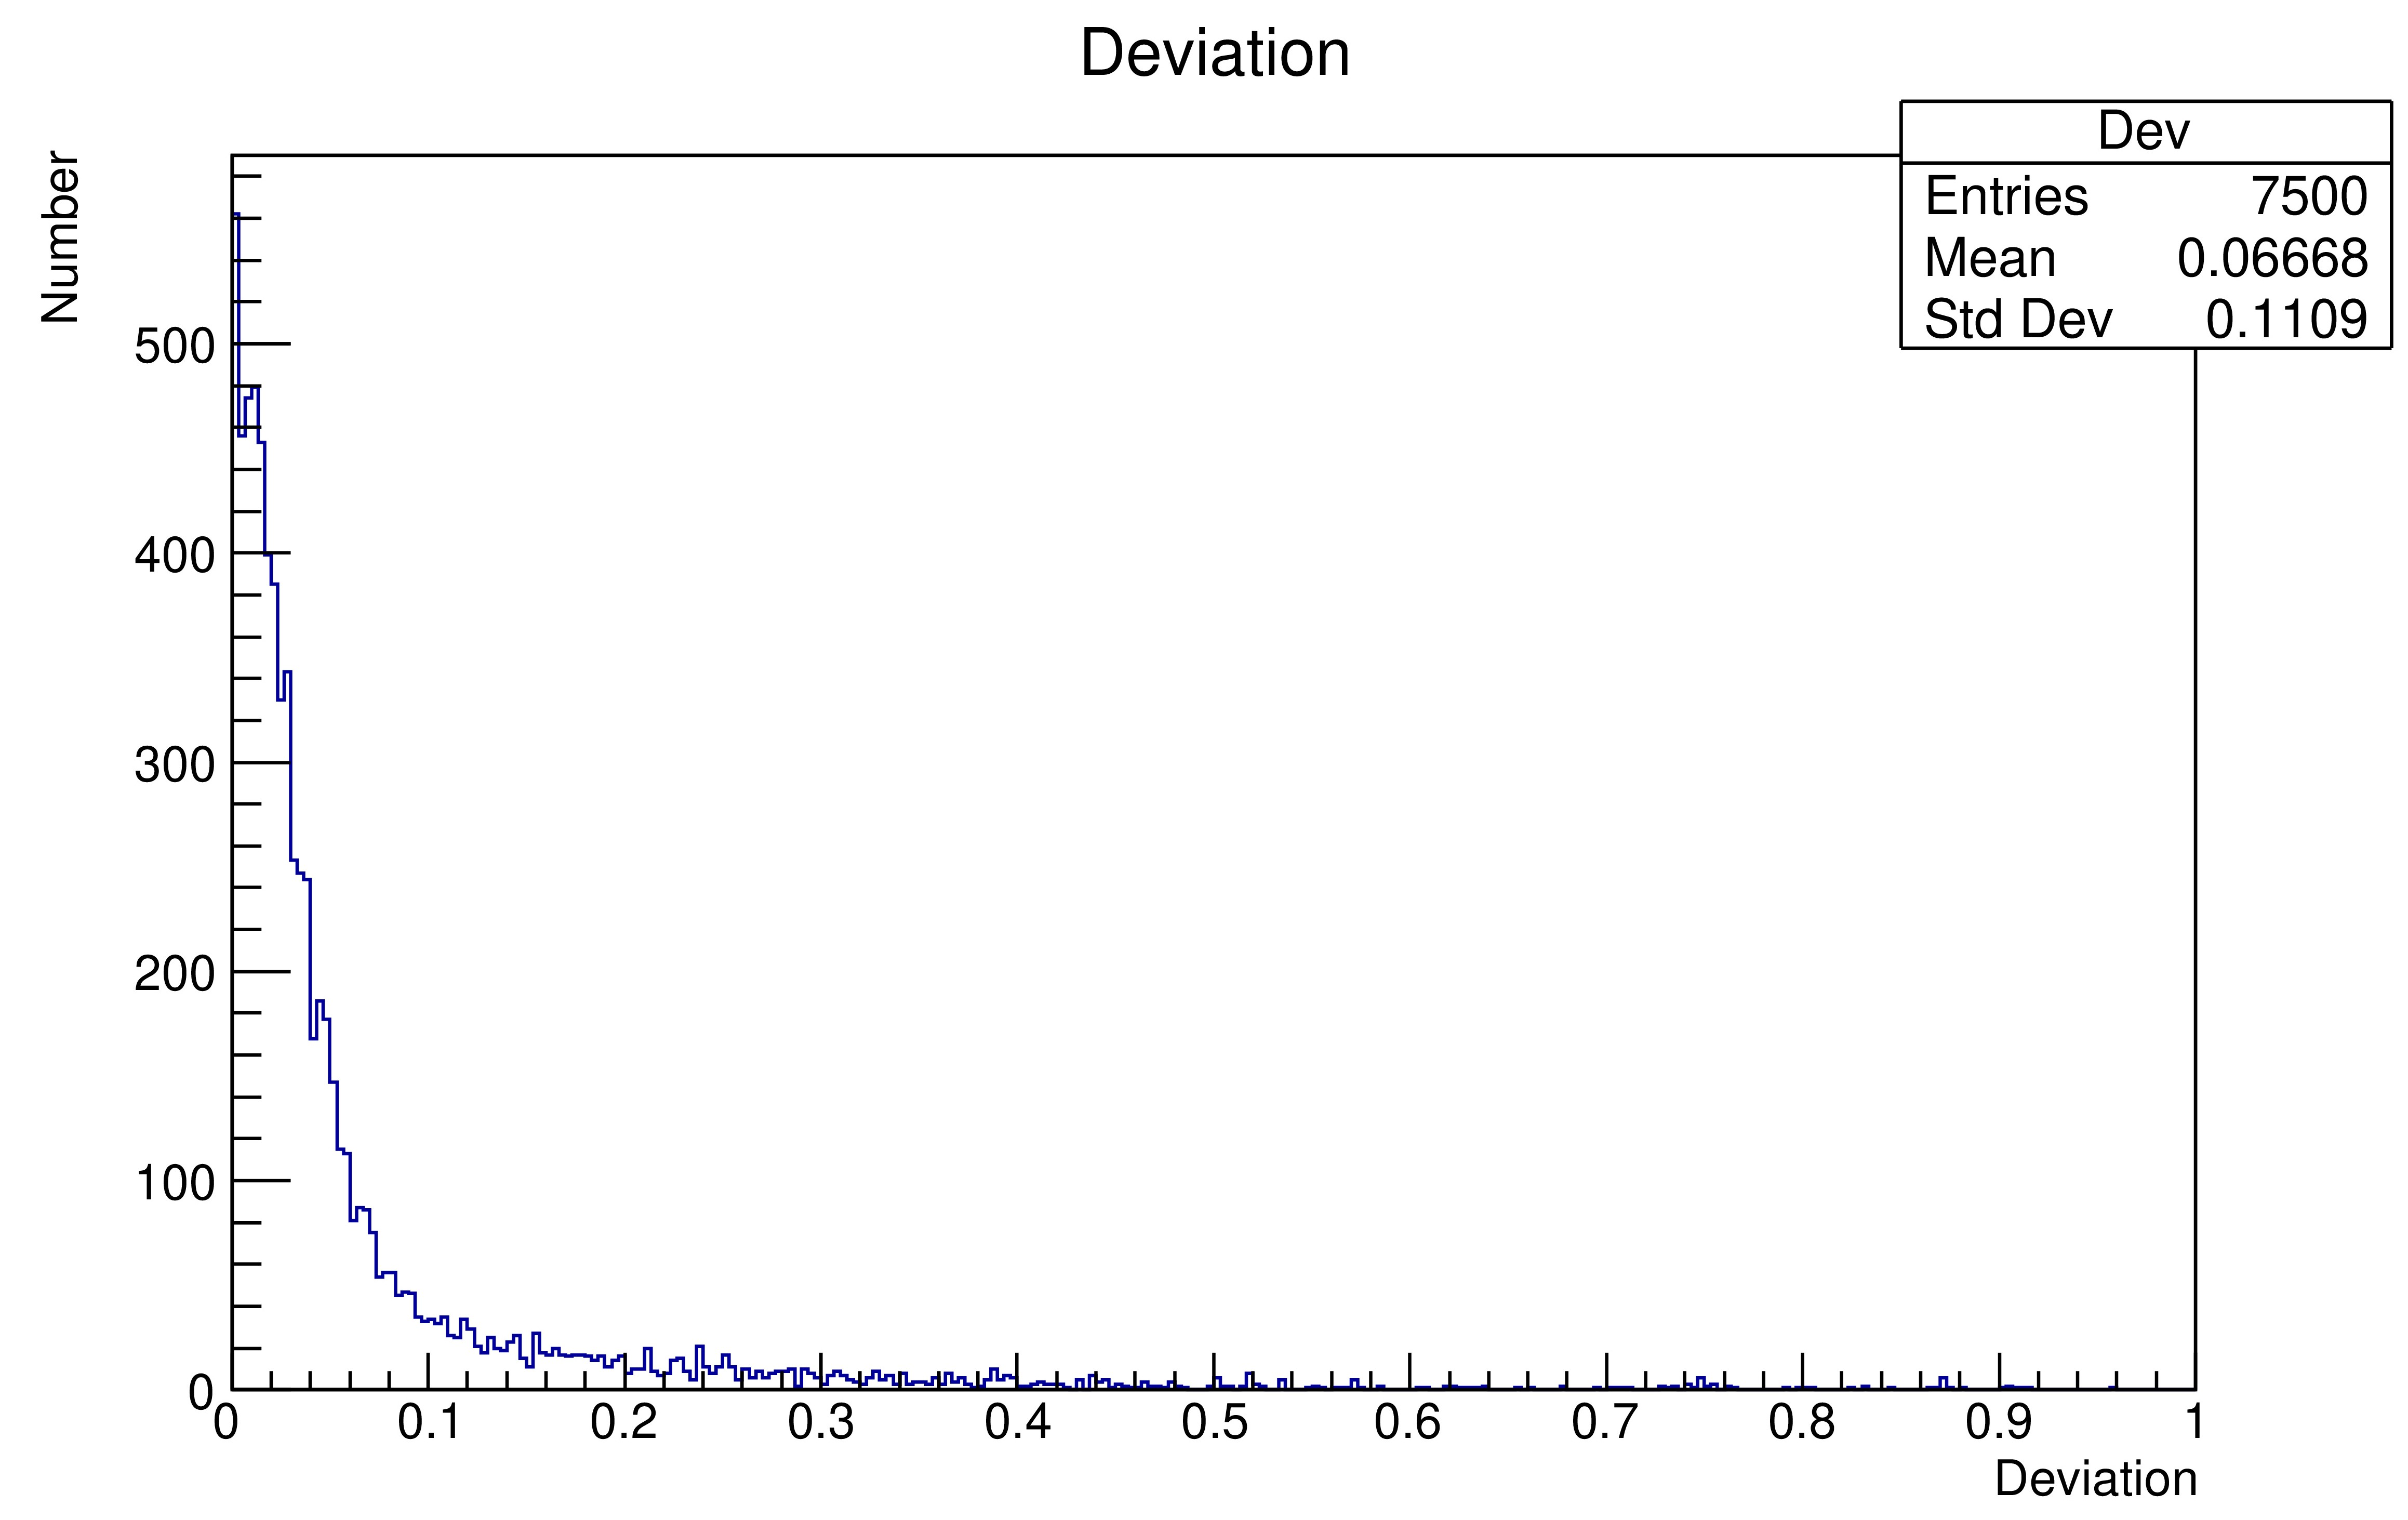
\includegraphics[width=0.45\textwidth]{figures/RD/Kriging.jpg}\label{fig:exgr7}}
        \subfigure[本论文提出]{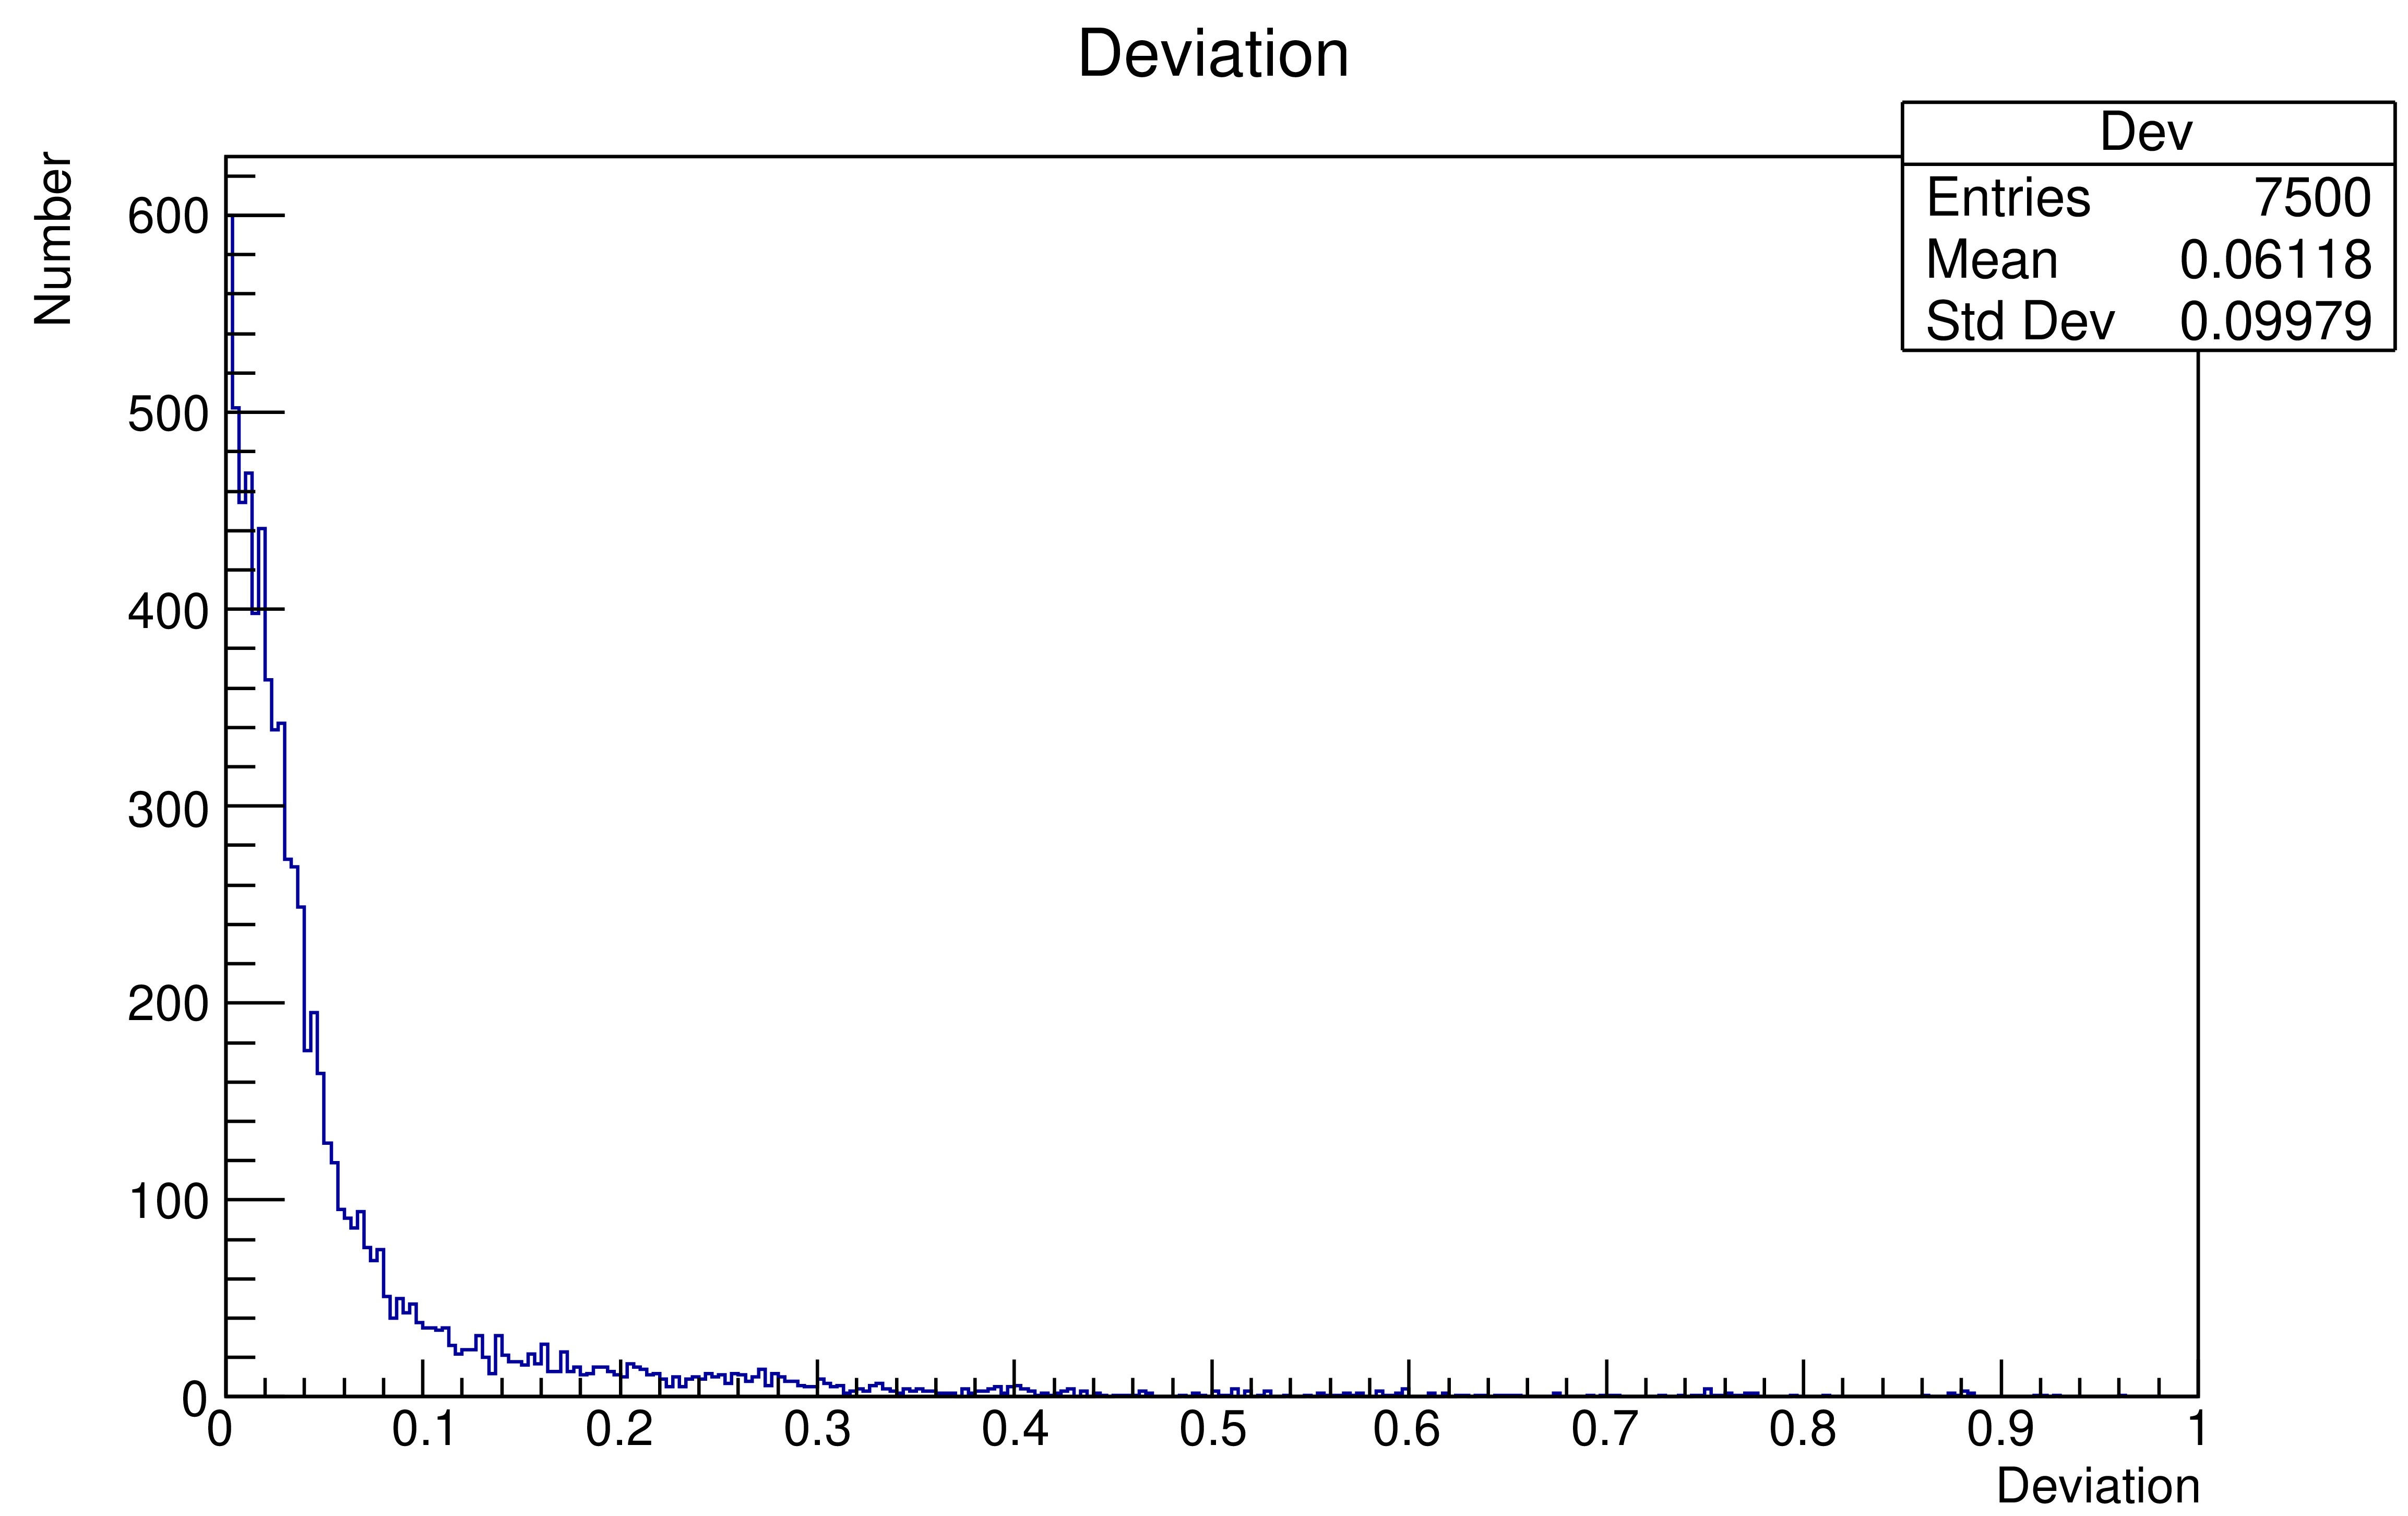
\includegraphics[width=0.45\textwidth]{figures/RD/Innvation.jpg}\label{fig:exgc7}}
    \end{figure}
\end{frame}

\begin{frame}
    \frametitle{重构时间比较}
    \begin{table}[htbp]
        \centering
        \caption{\label{tab:test4}不同重构插值方法下辐射场重构时间比较}
        \begin{tabular}{lccc}
            \toprule
            空间辐射场类型   & 多层B样条(s) & 克里金(s) & 本论文(s) \\
            \midrule
            单点源无屏蔽空间 & 1.20776      & 0.000233  & 0.001025  \\
            多点源无屏蔽空间 & 2.02339      & 0.000188  & 0.001567  \\
            单点源有屏蔽空间 & 1.9229       & 0.000169  & 0.00236   \\
            多点源有屏蔽空间 & 1.93904      & 0.000223  & 0.001668  \\
            \bottomrule
        \end{tabular}
        \label{不同重构插值方法下辐射场重构时间比较}
    \end{table}
\end{frame}

\section{论文总结}

\subsection{论文完成主要工作}
\begin{frame}
    \frametitle{论文完成主要工作}
    \begin{enumerate}
        \item 基于多层次B样条插值和克里金插值提出一种空间辐射场三维重构方法,能够实现三维区域内散乱数据重构。
        \item 利用蒙特卡洛应用软件包Geant4模拟四种不同类型辐射场,通过对该四种辐射场进行重构,分别探究源项数量、辐射场空间状况以及重构测点数量对辐射场插值重构的影响。
        \item 将本论文提出的辐射场重构方法与多层B样条插值重构方法、克里金插值重构方法相比较。
    \end{enumerate}
\end{frame}

\subsection{下一步的工作建议}
\begin{frame}
    \frametitle{下一步的工作建议}
    \begin{enumerate}
        \item 将本文提出的辐射场插值重构方法在实际辐射场中进行应用,分析其在实际应用中的偏差大小,进一步验证其可行性;
        \item 改进本论文辐射场插值重构中多层B样条插值和克里金插值的结合方式,将其比重与辐射场分布梯度关联,提高其插值精度;
        \item 引入更多的插值重构方法,例如有限元法、三角划分法等等,分析以上方法在哪些辐射场区域分布下精度较高,将其进行组合;
        \item 将机器学习算法应用于辐射场重构领域中,分析其可行性并与现有重构方法对比。
    \end{enumerate}
\end{frame}

\begin{frame}
    \Huge{\centerline{谢谢!}}
\end{frame}

\end{document}